\begin{section}{Prueba de concepto}
Para no afectar al funcionamiento del servicio proporcionado por el CITIC y para mostrar y probar las capacidades de VMware Cloud Foundation, en lugar de utilizar un entorno real el proyecto se lleva a cabo en un entorno aislado de prestaciones reducidas. La instalación de VMware Cloud Foundation se realiza con la herramienta VMware Lab Constructor (VLC)\footnote{Se utiliza la versión 4.0.1 del instalador.}, que genera de forma automatizada una infraestructura embebida basada en el diseño de VMware Cloud Foundation propuesto por VMware sobre la cual despliega cada uno de los componentes para simular un entorno real. Una vez generado se instalarán las aplicaciones necesarias para gestionar los usuarios del sistema y el servicio de aprovisionamiento.

\begin{subsection}{Preparación}
  \begin{subsubsection}{Host ESXi}  
  
  Como base para la instalación se utiliza un servidor físico con el hipervisor ESXi instalado que aunque no cumpla con alguno de requisitos mínimos de VMware Cloud Foundation, no aporta gran rendimiento pero si permite crear un entorno funcional a modo de prueba. Este host cuenta con una memoria RAM de 128 GB, una CPU de 28,8 GHz y un \textit{datastore} con discos SSD con 2 TB de capacidad. Cuenta con dos interfaces físicas, una que conecta al host con el \textit{datastore} y otra a la que se conectan dos redes, una llamada \textit{Management Network} que permite acceder al host desde una VM para gestionarlo, y otra llamada \textit{VM Network} donde se conectan todas las VMs generadas por VLC y de los servicios que dan soporte a los componentes de VMware Cloud Foundation.
  \end{subsubsection}
  \begin{subsubsection}{Servicios}
    Todos los servicios requeridos por VMware Cloud Foundation se despliegan sobre el mismo servidor en forma de VMs. Una de las VMs es Windows Server 2016 que contiene un servidor DNS, un servidor NTP, un servidor Active Directory, un servidor SMTP y ejerce también como Certificate Authority. Otra VM contiene el sistema operativo VyOS que funciona como un router virtual y como servidor DHCP. Una última VM con Windows 10\footnote{Se refiere a ella como \textit{Jump Host}.} se requiere para ejecutar VLC y acceder al entorno embebido generado por VLC.
    El servidor DNS contiene los \textit{hostnames} y sus respectivas direcciones IP de todas las VMs, tanto las que residen dentro del host físico como las que se alojan dentro del entorno embebido generado por la herramienta VLC. Este servidor DNS implementa un único dominio que se denomina \textit{pesci.domain}. El servidor Active Directory proporciona almacena usuarios y grupos de usuarios requeridos para establecer roles y proporcionar acceso a los componentes y servicios de VMware Cloud Foundation. Se utiliza este servidor de usuarios en lugar del directorio real de la UDC para evitar posibles problemas del servicio. El router VyOS tiene configuradas todas las subredes y VLANs que VMware Cloud Foundation utiliza en la capa L3 de la infraestructura física y proporciona acceso a Internet, en las cuatro interfaces que conectan con las instancias de VMware NSX-T Edge utiliza enrutamiento dinámico BGP. El servidor DHCP asigna una dirección IP a cada TEP de cada host ESXi.    
  \end{subsubsection}
  
  \begin{subsubsection}{VMware Lab Constructor}
    VLC genera en el host ESXi cuatro VMs que representan cuatro hosts ESXi. posteriormente, dentro de estos hosts VLC inicia la creación del \textit{management domain} de esta infraestructura embebida incluyendo todos los componentes de VMware Cloud Foundation. El diseño y configuración generados se describirá en las siguientes secciones.
    \begin{figure}[h!]
      \centering
      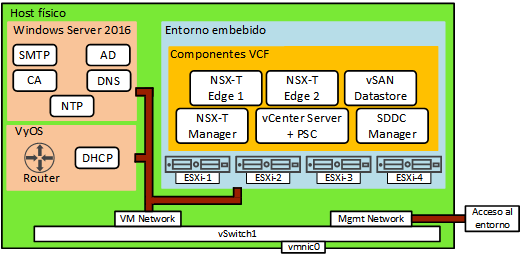
\includegraphics[width=0.6\textwidth]{imaxes/pruebaconcepto/hostFisico.png}
      \caption{Muestra la estructura generada por el instalador VLC. Cuatro hosts ESXi embebidos con los componentes de VMware Cloud Foundation cuyo tráfico circula a través del \textit{port group} VM Network.}
      \label{fig:estructura-generada-por-VLC}
    \end{figure}
    \begin{figure}[h]
      \centering
      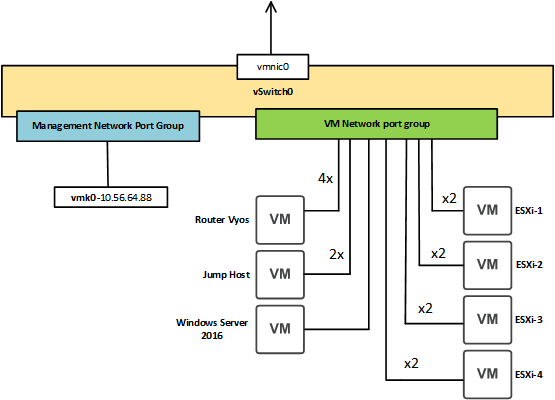
\includegraphics[width=0.6\textwidth]{imaxes/pruebaconcepto/vSwitch0HostFisico.png}
      \caption{Muestra las VMs que están funcionando sobre el host físico y que representan los componentes de la infraestructura física de un SDDC real, junto con el número de interfaces que se utilizan en cada una. Cada host ESXi generado por VLC cuenta con dos interfaces de red. El router VyOS, Jump Host y Windows Server 2016 se configuran antes del despliegue de VMware Cloud Foundation con VLC y se comunican con el entorno generado por VLC a través del \textit{port group} VM Network. El \textit{port group} Management Network se utiliza para acceder a la configuración del host físico a través de la dirección que se indica. Se utiliza la interfaz vmnic0 del host como salida del tráfico generado por el vSwitch0.}
      \label{fig:VMs-alojadas-host-fisico}
    \end{figure}
    \begin{figure}[h]
      \centering
      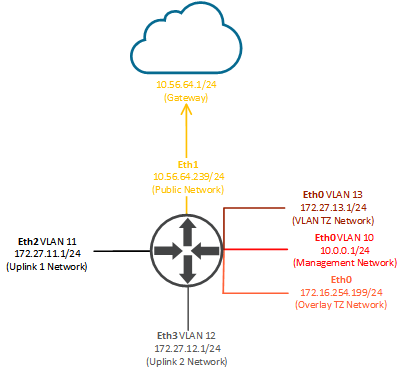
\includegraphics[width=0.4\textwidth]{imaxes/pruebaconcepto/RouterFisicoL3.png}
      \caption{Muestra la configuración del router VyOS. Cada una de las interfaces se debe configurar antes del despliegue de VCF. Todas usan MTU de 8940 Bytes. 
      En las interfaces Eth2 y Eth3 el router utiliza enrutamiento dinámico BGP donde el AS local es 65001 y el AS remoto es AS 65003, configurado para anunciar a sus vecinos la red 10.0.0.0/24 Management Network. Las direcciones configuradas como \textit{neighbour} son: 172.27.11.2, 172.27.11.3, 172.27.12.2 y 172.27.12.3. En la dirección IP 172.27.254.199 de la interfaz eth0, el router proporciona un servidor DHCP que asigna direcciones IP en el rango 172.16.254.0 - 172.16.254.100.}
      \label{fig:interfaces-router-fisico-L3}
    \end{figure}
    \begin{figure}[h]
      \centering
      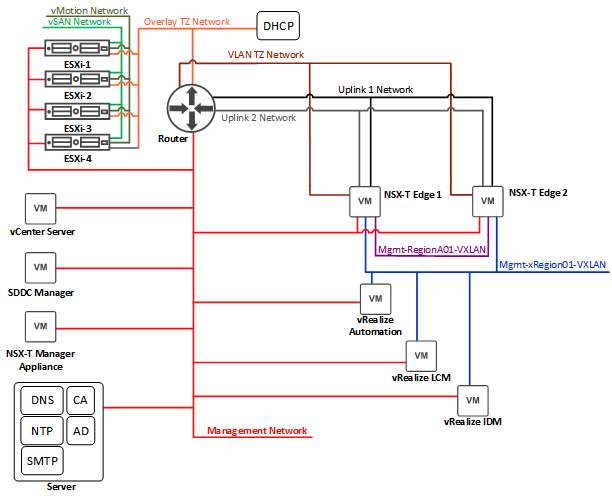
\includegraphics[width=0.6\textwidth]{imaxes/pruebaconcepto/RedDesdeDentro.png}
      \caption{Muestra todos los componentes de VMware Cloud Foundation desplegados por VLC, como se conectan con los distintos servicios de red y a que redes se conectan. Las redes Mgmt-xRegion01-VXLAN y Mgmt-Region01A-VXLAN se corresponden a redes virtuales gestionadas por VMware NSX-T que no requieren ninguna configuración adicional en la capa 3 de la infraestructura física (esto se verá con detalle en el apartado de diseño de VMWare NSX-T).}
      \label{fig:red-L3-infraestructura-fisica}
    \end{figure}
    \FloatBarrier
  \end{subsubsection}
  
\end{subsection}
    %%%%%DISEÑO ARQ. VIRTUAL
\begin{subsection}{Diseño y configuración del Management Domain}
    
    % Esta capa virtual provee infraestructura de almacenamiento, red y cómputo definida por software a través de servicios. En el modelo de despliegue consolidado de VMware Cloud Foundation, todos sus servicios y componentes se encuentran dentro de un mismo cluster (solo una AZ) dentro de la infraestructura, mientras que en el modelo estándar los servicios y componentes de gestión de la infraestructura están situados en clusters distintos (pueden estar en AZ distintas), todos sus componentes se encuentran agrupados en un mismo cluster.
    
    
    
    \subsubsection{Diseño de VMware vCenter Server}
    El componente VMware vCenter Server es el punto de acceso y de control de todas las máquinas virtuales localizados en los hosts ESXi que forman parte de su dominio. En el entorno desplegado se utiliza una instancia de VMware vCenter Server para controlar el \textit{management domain}, se denomina \textit{vcenter-mgmt}. Esta instancia de vCenter Server contiene un dominio que con un cluster vSphere formado por los cuatro hosts ESXi desplegados por VLC, estos se denominan respectivamente \textit{esxi-1}, \textit{esxi-2}, \textit{esxi-3} y \textit{esxi-4}. En vCenter Server se gestionan los recursos de las VMs de cada componente, se monitorizan los recursos, permite la creación y asignación de roles, permisos y usuarios, aisla las redes que usan los recursos que controla de otras instancias de vCenter Server, permite gestionar los grupos de discos de almacenamiento de cada host ESXi que forman el \textit{datastore} de VMware vSAN, administrar las redes a las que se conecta cada componente, en definitiva, VMware vCenter Server es el punto desde el cual se controlan los recursos que utiliza cada componente. Además, incluye el componente PSC que controla el dominio de autenticación de VMware vSphere SSO Domain denominado \textit{local}. Desde vCenter Server también se controlan las características de alta disponibilidad y recuperación ante fallos de VMware vSphere como se verá a continuación. El acceso a vCenter Server se hace a través del componente web vSphere Client.
    \begin{figure}[h]
      \centering
      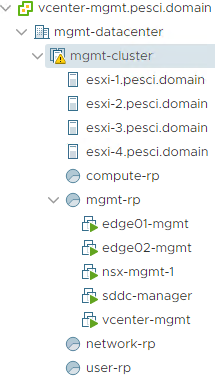
\includegraphics[width=0.2\textwidth]{imaxes/pruebaconcepto/clusterVCenterServer.png}
      \caption{Muestra el dominio (\textit{vcenter-mgmt.pesci.domain} de la instancia de vCenter Server y el cluster vSphere (\textit{mgmt-cluster}) donde se alojan los componentes del \textit{management domain}. Incluye cuatro hosts ESXi y cuatro \textit{resource pools}, uno de ellos contiene las VMs de los componentes dedicados a este \textit{management domain}.}
      \label{fig:cluster-vCenter-Server}
    \end{figure}
    \FloatBarrier
    %  Con vCenter Server se simplifica la escalabilidad del SDDC, la gestión de actualizaciones para los componentes es más sencilla, permite determinar roles específicos y responsabilidades y permite aislar las redes de otras instancias de vCenter Server. Además, para gestionar vSpehere SSO Domain, VMware vCenter Server contiene embebido el componente PSC con todos los servicios necesarios. 
    %  En caso de que existan varios \textit{Workload Domain} se puede habilitar el modo \textit{Enhanced Linked Mode} para poder gestionar todas las instancias de vCenter Server de forma centralizada desde un único vSphere Client.
    % Por lo anterior, en el \textit{management domain} se despliega una instancia de VMware vCenter Server que incluye un cluster de VMware vSphere.
    
    \begin{subsubsection}{Diseño almacenamiento VMware vSAN}
      El almacenamiento del \textit{management domain} desplegado, está implementado con VMwware vSAN. Los cuatro hosts ESXi contienen cuatro grupos de discos cada uno con configuración All-Flash. Como hay cuatro hosts participantes, soporta el fallo de un host lo cual permite dejar hosts fuera de servicio para tareas de mantenimiento. Esto es posible gracias a que con FTT (\textit{Failures-To-Tolerate}) igual a 1 se mantiene la redundancia de los datos almacenados en el \textit{datasotore}, en uno de los hosts. Cada grupo de discos cuenta con cuatro discos uno de ellos para caché, 16 discos en total. Para hacer disponible este servicio de almacenamiento, todos los hosts deben estar conectados a la subred generada para VMware vSAN y utilizar una VLAN para separar su tráfico.
    \end{subsubsection}
        
    \begin{subsubsection}{Diseño cluster VMware vSphere}
    Dentro de un \textit{workload domain} pueden existir varios clusters vSphere con diferentes características según su finalidad. Los hosts ESXi que lo forman pueden ser de diferentes tamaños teniendo en cuenta que se pueden usar menos hosts ESXi de mayor capacidad o más hosts con menores prestaciones, el coste de cada host ESXi, el uso que se le va a dar al cluster y las características máximas y mínimas del cluster vSphere. Para el \textit{management domain} se utiliza un único cluster vSphere con de 4 hosts de los cuales se reserva un host para proveer redundancia. Todos los hosts ESXi cuenta con 64GB de memoria RAM menos uno que tiene 32 GB, y 19.9GHz de CPU. Dentro del cluster hay que configurar los servicios vSphere HA y vSphere DRS para proteger los componentes del SDDC. La configuración que se establece en el \textit{management domain} es la siguiente:
    % En caso de que el \textit{management domain} esté extendido en dos AZ entonces se requieren 4 hosts en cada AZ para proporcionar redundancia y disponibilidad en caso de caída de una de las AZ.
   
    \begin{itemize}
        \item \textbf{vSphere High Availability}: en este servicio la propiedad \textit{Admission Control Policy} permite establecer la cantidad recursos reservados en caso de fallo y como se establece el cálculo de esos recursos. En el \textit{management domain} se configura para el fallo de al menos un host y reserva de recursos según un porcentaje, reservando así el 25\% de la CPU y el 30\% de la memoria RAM ya que funciona mejor cuando las VM usan mucha CPU y memoria. La otra propiedad que se debe habilitar para el correcto funcionamiento del servicio es \textit{VM and Application Monitoring}, que se encarga de reiniciar las VM en caso de caída.
        % que puede ser según el número hosts que pueden fallar en el cluster, según un porcentaje de reserva de rescursos o especificando el host donde se recolocan las VM del host caído.  RAM.  
        \item \textbf{vSphere DRS}: este servicio permite migrar VMs de un host ESXi a otro dentro del mismo cluster vSphere para equilibrar la carga de trabajo y mantener las VMs activas en caso de caída de alguno de los hosts. se activa usando la opción por defecto \textit{Fully Automated} ya que aporta el mejor balance entre consumo de recursos y migraciones de VM innecesarias. Adicionalmente se pueden establecer reglas para determinar reglas de orden de encendido sobre grupos de VM. 
        %En caso de que exista más de una AZ, se deben crear grupos de VM y de hosts de cada AZ para luego implementar reglas de afinidad para que las VM de una AZ no sean migradas a otra AZ ya que esto puede afectar al rendimiento de la VM. 
    \end{itemize}
    % En el modelo consolidado se debe crear un único cluster con un mínimo de cuatro hosts ESXi ya que uno de los hosts se utiliza para asegurar la disponibilidad del almacenamiento vSAN cuando hay algún host inactivo. Este modelo proporciona capacidad de un único fallo por cluster.
    \end{subsubsection}
    \subsubsection{Diseño de red para el cluster vSphere}
    Si bien en VMware Cloud Foundation existe VMware NSX-T, un componente dedicado únicamente a la administración de la red del SDDC, es desde VMware vSphere dónde se encuentran los elementos para establecer redes que separen cada tipo de tráfico de los componentes del SDDC. Estas redes se configuran en base a los siguientes aspectos:
    \begin{itemize}
        \item Separar el tráfico de cada servicio para mejorar la eficiencia de la red y la seguridad. Así se puede ajustar las características de cada red, como el ancho de banda o la latencia, a las necesidades de cada servicio.
        \item Utilizar un único vSphere Distributed Switch por cluster donde se añade un \textit{port groups} por cada servicio.
        % \item Mejorar el rendimiento usando NICs de tipo VMXNET3 en las máquinas virtuales.
        \item Las NICs físicas de cada host ESXi conectados a un mismo vSphere Distributed Switch están conectadas también a la misma red física.
        % \item Aquellas redes que se dedican a servicios de la infraestructura deben estar configuradas con puertos tipo \textit{vmkernel}.
    \end{itemize}
    Para el \textit{management domain} del SDDC se crea un único vSphere Distributed Switch llamado \textit{sddc-vds01} con la siguiente configuración:
    \begin{itemize}
        
        \item Se establece un MTU igual 9000 Bytes para permitir el tráfico de \textit{jumbo frames} ya que son requeridos por algunos de los servicios.
        
        \item Se habilita el servicio \textit{Network I/O} que permite establecer un nivel de prioridad a cada tipo de tráfico. Esto se realiza estableciendo limites de ancho de banda, políticas de balanceo de carga y reserva de recursos para un tipo de tráfico asociado a un servicio. Por cada tipo de tráfico hay cuatro aspectos que se pueden configurar que son \textit{Shares} (indica el \% de ancho de banda que se le da a un tipo de tráfico, el tipo de tráfico que tenga un mayor valor en \textit{Shares} tendrá más prioridad a la hora de usar los recursos), \textit{Reservation} (indica el valor de ancho de banda que se reserva para el tipo de tráfico) y \textit{Limit} (establece un valor máximo para el ancho de banda de un tipo de tráfico). En el \textit{management domain} los tipos de tráfico más relevantes que se deben configurar son los siguientes:
        \begin{itemize}
          \item \textit{Management Traffic}: el valor \textit{Shares} se establece al 50\% (\textit{Normal}) lo cual le da mayor prioridad que el resto de tipos. El resto de valores no se modifican.
          \item \textit{vSphere vMotion Traffic}: el valor \textit{Shares} se establece al 25\% (\textit{Low}) ya que durante el estado normal del entorno este tipo de tráfico no es muy importante. El resto de valores no se modifican.
          \item \textit{vSAN Traffic}: el valor \textit{Shares} se establece al 100\% (\textit{High}) para garantizar que este servicio recibe la cantidad de ancho de banda que necesita. El resto de valores no se modifican.
          \item \textit{Virtual Machine Traffic}: el valor \textit{Shares} se establece al 100\% (\textit{High}) para garantizar que las VMs siempre tienen acceso a la red ya que son una parte importante del SDDC. El resto de valores no se modifican.
        \end{itemize}
        
        \item Para detectar errores de compatibilidad entre la configuración del vSphere Distributed Switch y la red física se habilita el servicio \textit{Health Check}. Este se encarga de comprobar si la configuración de cada VLAN y MTU se adapta a la configuración de la capa física.
        
        \item Como puertos de salida \textit{Uplink} se configuran las interfaces físicas \textit{vmnic0} y \textit{vmnic1}. Como vDS es un componente distribuído, en cada host se usarán ambas interfaces de red como \textit{uplinks}.
        
    \end{itemize}
    En este vSpehere Distributed Switch para el \textit{management domain} se configuran los siguientes \textit{port groups}, que son de tipo \textit{Distributed port group} y de tipo \textit{Uplink port group}:
    \begin{itemize}
           
            \item \textbf{Management port group}: es un \textit{Distributed port group} que comunica a todos los hosts ESXi entre si y transmite el tráfico entre los diferentes componentes de VMware Cloud Foundation, es decir, por este \textit{port group} circulan los comandos de configuración y gestión que los componentes del SDDC se envían entre ellos. Con el nombre \textit{sddc-vds01-mgmt}, en él están configurados los cuatro hosts ESXi y las VMs \textit{vcenter-mgmt}, \textit{sddc-manager}, \textit{nsx-mgmt-1},\textit{edge01-mgmt} y \textit{edge02-mgmt} bajo la subred con IP 10.0.0.0, con máscara de red 255.255.255.0, con VLAN 10 y con MTU igual a 1500 Bytes. Esta red debe ser configurada también en la infraestructura física.
            
            \item \textbf{vMotion port group}: es un \textit{Distributed port group} que está dedicado al tráfico del componente vSphere vMotion para realizar las migraciones de máquinas virtuales de un host a otro. Con el nombre \textit{sddc-vds01-vmotion}, en él están configurados los 4 hosts bajo la subred con IP 10.0.4.0, con máscara de red 255.255.255.0, con VLAN 10 y con MTU igual a 8940 Bytes.
            
            \item \textbf{vSAN port group}: es un \textit{Distributed port group} que está dedicado al servicio de almacenamiento VMware vSAN y por él los hosts acceden al almacenamiento del SDDC. Con el nombre \textit{sddc-vds01-vsan}, en él están configurados los 4 hosts bajo la subred con IP 10.0.8.0, con máscara de red 255.255.255.0, con VLAN 10 y con MTU igual a 8940 Bytes.
            
            \item \textbf{Edge Uplink port group}: es un \textit{Distributed port group} dedicado a las conexiones del component NSX-T Edge que se dedica a dar acceso a determinados servicios y para proporcionar a otros \textit{workload domain} conexión con la red externa. Están gestionados por VMware NSX-T ya que dan servicio a sus componentes. En el entorno existen dos \textit{port groups} para proporcionar redundancia y alta dispobilidad, uno llamado \textit{sddc-edge-uplink01} cuyas instancias están configuradas bajo la red con IP 172.27.11.0 y con máscara de red 255.255.255.0, y otro llamado \textit{sddc-edge-uplink02} cuyas instancias están configuradas bajo la red con IP 172.27.12.0 y máscara de red 255.255.255.0. Ambos \textit{port groups} están configurados como VLAN Trunk (por ellos puede circular tráfico de cualquier VLAN) y tienen un MTU de 8940 Bytes. En los dos están configuradas dos VM llamadas \textit{edge01-mgmt} y \textit{edge02-mgmt}. Estas dos redes también se deben configurar en la infraestructura física.
            
            \item \textbf{Uplink port group}: se trata de un \textit{Uplink port group} al que se le asignan las NICs físicas de cada host para establecer políticas sobre el tráfico que se dirige desde los hosts y VMs hacia fuera del vSphere Distributed Switch. Con el nombre \textit{sddc-vds01-DVUplinks-10}, en él están configuradas las dos NICs físicas de cada host, cada una en una interfaz \textit{uplink}.
            
    \end{itemize}
    \begin{figure}[h]
      \centering
      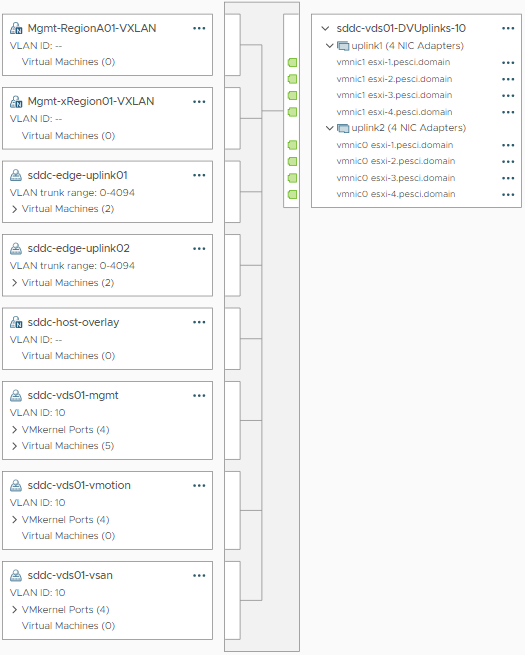
\includegraphics[width=0.4\textwidth]{imaxes/pruebaconcepto/distributedSwitchEntornoFinal.png}
      \caption{Muestra todos los \textit{Distributed Port Groups} y \textit{Uplink port group} que se alojan en el vSphere Distributed Switch (\textit{sddc-vds01}) dedicado al \textit{management domain}. En el \textit{port group} \textit{sddc-vds01-DVUplinks-10} se muestra como a cada interfaz \textit{uplink} se mapea una interfaz física (vmnic) de cada host ESXi. Los \textit{port groups} \textit{mgmt-Region01A-VXLAN}, \textit{mgmt-xRegion01-VXLAN} y \textit{sddc-host-overlay} son generados y administrados por el componente VMware NSX-T como se explicará más adelante. Cada \textit{port group} informa de cuantas VMs y hosts ESXi tiene conectados.}
      \label{fig:port-groups-vSwitch-vSphere}
    \end{figure}
    \FloatBarrier
    La configuración que se aplica a cada \textit{Distributed port group} descrito anteriormente es la siguiente:
    \begin{itemize}
      \item \textit{Port binding}: permite indidcar como se gestionan los puertos de un \textit{port group} cuando se añade o elimina una VM. Tiene dos opciones de configuración, la primera se denomina \textit{Static Port Binding} y su función consiste en asignar un puerto dentro del \textit{port group} a la VM que se conecta y solo se elimina cuando la VM es borrada. La segunda opción se denomina \textit{Ephemeral Port Binding} y consiste en que el puerto se asigna a la VM cuando esta se enciende y se elimina cuando se apaga o elimina. Para los \textit{port groups} \textit{sddc-vds01-vsan} y \textit{sddc-vds01-vmotion} se configura la opción \textit{Static Port Binding} ya que así se asegura que las VMs se conectan siempre al mismo puerto lo cual permite mantener datos históricos y hacer monitoreo a nivel de puerto. Para los \textit{port group} \textit{sddc-vds01-mgmt}, \textit{sddc-edge-uplink01} y \textit{sddc-edge-uplink02} se configura la opción \textit{Ephemeral Port Binding} ya que como el tráfico que circula por ellos es el que gestiona todos los componentes y da acceso a otras redes etonces se elimina la dependencia del estado de vCenter Server permitiendo que la comunicación continúe aunque vCenter Server no se encuentre operativo.
    
      \item \textit{Load Balancing}: indica como se distribuye el tráfico de salida de cada VM/host que se encuentran en el \textit{port group} entre las NICs físicas. Se selecciona \textit{Route based on physical NIC load}, es decir, el tráfico de una VM se transmite por una única NIC por lo que si esa NIC física está saturada, se asignará otra NIC física a la VM.
      
      \item \textit{Network failure detection}: esta opción permite establecer como debe determinar el \textit{port group} que alguna de las NICs físicas está fuera de servicio. Se selecciona \textit{Link status only} para que esto se determine según el estado que le transmite la NIC física, así se pueden detectar los fallos que ocurren en la red física.
      
      \item \textit{Notify switches}: se habilita para permitir a los host enviar \textit{frames} a los switches físicos para que estos conozcan la localización de las VM que están funcionando en cada host.
      
      \item \textit{Failback}: permite determinar como se reactiva una NIC cuando esta se recupera de un fallo. Se habilita para establecer que la NIC se marcará como activa inmediatamente después de que se haya recuperado. Esta opción se debería desactivar en caso de que el estado de la NIC sea inestable.
      
      \item \textit{Failover Order}: permite determinar que uplinks se deben utilizar, los que se seleccionan como \textit{active} son los que se utilizarán por defecto, los que se seleccionan como \textit{stand by} se usarán cuando los uplinks marcados como \textit{active} se encuentren desactivados. Se seleccionan las dos interfaces \textit{uplink} disponibles en el estado \textit{active}. Para el \textit{port group} \textit{sddc-edge-uplink01} se selecciona la interfaz \textit{uplink1} como activa y se deja sin usar la interfaz \textit{uplink2}, mientras que se configura de forma contraria en el \textit{port group} \textit{sddc-edge-uplink02}.
    \end{itemize}
    
    
    %%%%%%%%%%%%%%%%%%%%%%%%%%%%%%%%%%%%%%%%%%%%
    \subsubsection{Diseño de la red del SDDC con VMware NSX-T}
    En un SDDC debe existir una red virtual, es decir, definida por software o también conocida como \textit{Software-Defined Network}. Esta red al estar construída con componentes de software, se desacopla de la red física sobre la que funciona lo que hace posible que se pueda modificar sin necesidad de cambiar la configuración en la capa física, reduciendo así la complejidad de la red física y el tiempo dedicado a la gestión de la misma. Además, este tipo de arquitectura habilita la posibilidad de implementar múltiples configuraciones de red en tiempo reducido proporcionando elasticidad y flexibilidad a la hora de administrar los recursos, tanto para el administrador como para el usuario final.
    El componente encargado de crear, configurar y administrar la red virtualizada del SDDC es VMware NSX-T que a su vez contiene otros componentes entre los que se dividen distintas responsabilidades y funciones, ya descritos anteriormente.
    
    %%%%% 1 - EXPLICACION DE LOS COMPONENTES DE NSX Y LOS QUE HAY EN EL ENTORNO
    %%%%% 2 - COMO SE DEBE CONFIGURAR LA CAPA FÍSICA Y COMO ESTÁ IMPLEMENTADA EN EL ENTORNO ( parte de esto ya está definido en la parte de red física, REVISAR) => Meter la descripción de lo físico con el resto (modificar ese apartado) [https://docs.vmware.com/en/VMware-Validated-Design/6.0/sddc-architecture-and-design-for-the-management-domain/GUID-C924E896-D9C4-47BF-91D5-DF72605EF63E.html]
    %%%%% 3 - REDES QUE HAY Y COMO SE EXTIENDEN ENTRE AZs
    %%%%% 4 - COMO FUNCIONAN LAS COMUNICACIONES (GENEVE, ROUTING ...)
    
    % En esta sección se describe como VMware Cloud Foundation abstrae la red física en un conjunto de recursos virtuales de red, utilizando los servicios de VMware NSX para crear una capa virtual independiente de la infraestructura física.
    Aunque se recomienda desplegar tres instancias de NSX-T Manager en el \textit{management domain}, VLC solo despliega una única instancia llamada \textit{nsx-mgmt-1} para mejorar el rendimiento del entorno. Además, VLC también genera dos instancias de NSX-T Edge que se denominan \textit{edge01-mgmt} y \textit{edge02-mgmt}. %cada conjunto de instancias de cada componente forman un cluster donde cada VM está protegida por las funcionalidades vSphere HA y vSphere DRS para proveer alta disponibilidad del servicio y migrar las VMs a otra ubicación en caso de caída de una AZ o de un host. 
    Estas VMs están conectadas al \textit{port group} \textit{sddc-vds01-mgmt} que les permite comunicarse entre ellas y con vCenter Server, además las instancias de NSX-T Edge también están conectadas a otros dos \textit{Distributed port group} llamados \textit{sddc-edge-uplink01} y \textit{sddc-edge-uplink02}. %Si existe más de una AZ, varios de los \textit{distributed port groups} se deben extender al resto de AZs para que en caso de que la primera AZ falle sus VMs se puedan migrar a otra AZ y sigan teniendo conectividad. Los \textit{port groups} que deberían estar extendidos en todas las AZ son el \textit{port group} \textit{sddc-vds01-mgmt} de cada AZ\footnote{Cada AZ tiene su propio \textit{Management port group}, entonces en cada AZ debe ser accesible el \textit{Management port group} del resto de AZs.}, los \textit{port group} \textit{sddc-edge-uplink01}, \textit{sddc-edge-uplink02} y \textit{port group} \textit{Edge Overlay}.
    
    Los elementos que utiliza VMware NSX-T para crear una red independiente de la configuración de la red física son \textit{Segment} y \textit{Transport Zone}. Con estos componentes VMware NSX-T puede crear túneles que definen redes de capa 2 sin necesidad de realizar ningún cambio en la configuración de la red física.
    \begin{itemize}
      \item \textbf{Transport Zone} (TZ): define el alcance de la red virtual. Pueden ser de dos tipos distintos, basada en VLAN o basada en Overlay. Una TZ se puede asignar a varios TN que tendrán acceso a los \textit{segments} que funcionen en esa TZ. Un TN se conecta a una TZ a través de un N-VDS los cuales pueden pueden estar conectados a varias TZ de tipo VLAN pero solo a una TZ de tipo Overlay al mismo tiempo.
      
      \item \textbf{Segment}: también llamado \textit{Logical Switch}, representa un dominio de broadcast de capa 2 que forma parte de una \textit{Transport Zone}. El tipo de tráfico puede ser VLAN u Overlay dependiendo de como se haya configurado la \textit{Transport Zone} de la que forma parte. Las VMs de cada TN se pueden conectar a los \textit{Segments} situados en las \textit{Transport Zones} a las que el host está conectado. Estas VMs se pueden comunicar con el resto de VMs conectadas al mismo \textit{Segment}.
       
    \end{itemize}
    Para gestionar las conexiones de cada TN, tanto para los nodos NSX-T Edge como para los hosts ESXi, VMware NSX-T introduce el componente llamado \textbf{NSX-T Virtual Distributed Switch} (N-VDS). Cada TN del \textit{management domain} posee un N-VDS, este elemento conecta sus interfaces a los \textit{segments} que se configuran en cada TN. Para el \textit{management domain} del entorno, VLC despliega dos \textit{transport zones} diferentes.
    \begin{figure}[h]
      \centering
      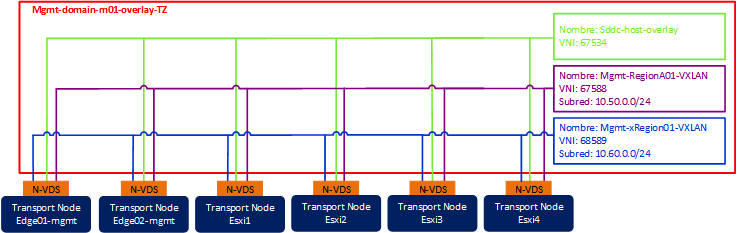
\includegraphics[width=1\textwidth]{imaxes/pruebaconcepto/OverlayTZSegments.png}
      \caption{Se muestra la \textit{transport zone} con el nombre \textit{mgmt-domain-m01-overlay-tz} de tipo Overlay. Está extendida en los seis TNs que hay en el \textit{management domain} y contiene tres \textit{segments}. El \textit{segment} \textit{mgmt-xRegion01-VXLAN} se utiliza para desplegar aplicaciones que deben ser accesibles desde todas las \textit{regions} que existan en el SDDC, es decir, la misma instancia de una aplicación está disponible desde varios puntos, así se reduce el consumo de recursos y aumenta la disponibilidad de esas aplicaciones ya que pueden migrar a distintas localizaciones según el estado de los recursos. El \textit{segment} \textit{mgmt-Region01A-VXLAN} tiene como finalidad alojar aplicaciones solo deben ser accesibles desde dentro de una misma \textit{region}. En estos dos \textit{segments} es donde se colocan los productos de VMware vRealize. Por último, el \textit{segment} \textit{sddc-host-overlay} es utilizado por los componentes de VMware NSX-T para comunicarse con y entre los diferentes TNs. VMware NSX-T genera en el vSphere vSwitch un \textit{port group} por cada \textit{segment} para poder conectar la VM de cada componente al \textit{port group} que le corresponda.}
      \label{fig:overlay-TZ-segments-NSXT}
    \end{figure}

    \begin{figure}[h]
      \centering
      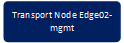
\includegraphics[width=1\textwidth]{imaxes/pruebaconcepto/VLANTZSegments.png}
       \caption{Muestra la\textit{transport zone} con el nombre \textit{sfo01-m01-edge-uplink-tz} de tipo VLAN. Está extendida en los dos TNs \textit{edge01-mgmt} y \textit{edge02-mgmt} y contiene dos \textit{segments}. Ambos \textit{segments} \textit{VCF-edge-mgmt-cluster-segment-11} y \textit{VCF-edge-mgmt-cluster-segment-12} son utilizados por las instancias de NSX-T Edge para transmitir el tráfico que proviene de los \textit{segments} donde se despliegan aplicaciones hacia la red externa (esto se explicará con más detalle). Estos \textit{segments} utilizan los \textit{port groups} \textit{trunk} del vSphere Switch para transmitir su tráfico hacia las interfaces de red físicas de cada host.}
      \label{fig:VLAN-TZ-segments-NSXT}
    \end{figure}

    \FloatBarrier
    %\begin{itemize}
      % \item \textit{mgmt-domain-m01-overlay-tz}:
      %   \begin{itemize}
      %     \item Tipo: Overlay
      %     \item Transport Nodes: \textit{edge01-mgmt}, \textit{edge02-mgmt}, \textit{esxi1}, \textit{esxi2}, \textit{esxi3} y \textit{esxi4}.
      %     \item Segments:
      %       \begin{itemize}
      %         \item \textit{mgmt-xRegion01-VXLAN}:
      %           \begin{itemize}
      %             \item VNI: 68589
      %             \item Subred: 10.60.0.0/24
      %             \item VMs: \textit{vrlcm} (10.60.0.60), \textit{vridm} (10.60.0.30)
      %             \item Descripción: se usa para desplegar las aplicaciones (algunos productos de VMware vRealize Suite lo utilizan) que deben ser accesibles desde todas las \textit{Regions} del SDDC, por lo tanto este \textit{segment} debe estar extendido en todo el entorno para que las VMs que se alojen en él puedan mantener la misma configuración de red independientemente del lugar físico donde se encuentren.
      %           \end{itemize}
      %         \item \textit{mgmt-Region01A-VXLAN}:
      %           \begin{itemize}
      %             \item VNI: 67588
      %             \item Subred: 10.50.0.0/24
      %             \item Descripción: su finalidad es alojar aplicaciones que sean accesibles desde una misma \textit{Region}. El alcance de estas aplicaciones está limitado a una \textit{Region} por lo tanto este \textit{segment} solo está extendido dentro de la misma.
      %           \end{itemize}
      %         \item \textit{sddc-host-overlay}:
      %           \begin{itemize}
      %             \item VNI: 67534
      %             \item Descripción: \textit{segment} usado por los componentes de VMware NSX-T para comunicarse entre los diferentes hosts ESXi.
      %           \end{itemize}
      %       \end{itemize}
      %   \end{itemize}
    %   \item \textit{sfo01-m01-edge-uplink-tz}:
    %     \begin{itemize}
    %       \item Tipo: VLAN
    %       \item Transport Nodes: \textit{edge01-mgmt} y \textit{edge02-mgmt}.
    %       \item Segments:
    %         \begin{itemize}
              
    %           \item \textit{VCF-edge-mgmt-cluster-segment-11}:
    %             \begin{itemize}
    %               \item VLAN: 11
    %               \item VMs: \textit{edge01-mgmt} (172.27.11.2/24) y \textit{edge02-mgmt} (172.27.11.3/24).
    %               \item Descripción: usado para transmitir el tráfico saliente hacia la red física.
    %             \end{itemize}
    %           \item \textit{VCF-edge-mgmt-cluster-segment-12}:
    %             \begin{itemize}
    %               \item VLAN: 12
    %               \item VMs: \textit{edge01-mgmt} (172.27.12.2/24) y \textit{edge02-mgmt} (172.27.12.3/24).
    %               \item Descripción: usado para transmitir el tráfico saliente hacia la red física.
    %             \end{itemize}
    %         \end{itemize}
    %       \end{itemize}
    % \end{itemize}
    
    Las TZ, tanto las basadas en Overlay como las basadas en VLAN, sirven para comunicar TNs que se encuentran en distintas partes de la infraestructura física (por ejemplo, en distintos racks) como si estuvieran situadas en el mismo dominio broadcast de capa 2 físico. 
    Aquellas que usan Overlay utilizan el protocolo Geneve para crear un túnel entre los puntos de origen y destino por el cual circula el tráfico generado por los \textit{segments} que pertenecen a esa TZ y que debe salir a la red física para alcanzar su destino. El protocolo Geneve añade una cabecera UDP a cada paquete Ethernet que generan los \textit{segments} cuando este sale del TN donde se generó hacia un TN situado en otra red física. La nueva cabecera incorpora un identificador llamado VNI y es único para cada \textit{segment} (cada \textit{segment} tiene su propio identificador VNI). 
    \begin{figure}[h]
      \centering
      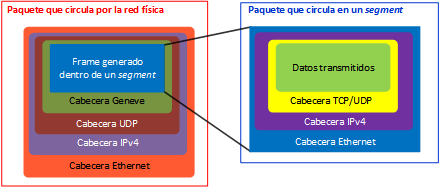
\includegraphics[width=1\textwidth]{imaxes/pruebaconcepto/FrameGeneve.png}
      \caption{Muestra las cabeceras que forman un paquete de red que pertenece a un \textit{segment} cuando este sale de un TN. Cuando el paquete que circula por la red virtual (contiene los datos que se transmiten y la información de las VMs origen y destino) tiene salir a la infraestructura física para alcanzar el destino, el \textit{transport node} añade la cabecera del protocolo Geneve con el identificador VNI correspondiente, una cabecera UDP con un puerto origen y destino establecidos por defecto, una cabecera IP con las direcciones IP origen y destino de los TN que se están comunicando, y una cabecera Ethernet donde se idican las direcciones MAC de los TN origen y destino. Así, dos VMs conectadas al mismo \textit{segment} pero alojadas en TNs de dominios broadcast diferentes, pueden comunicarse de forma transparente como si estuvieran conectadas directamente una con la otra en la misma subred.}
      \label{fig:Frame-Geneve-Segment-NSXT}
    \end{figure}
    \FloatBarrier
    % \begin{figure}[h]
    %   \centering
    %   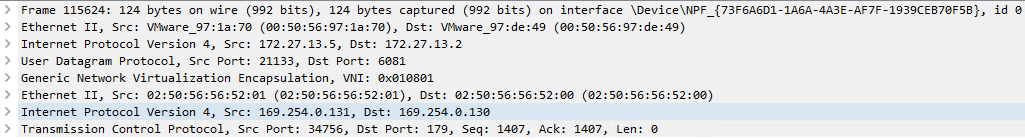
\includegraphics[width=1\textwidth]{imaxes/pruebaconcepto/FrameExampleGeneve.png}
    %   \caption{Cabeceras de un paquete capturado con el programa Wireshark que utiliza encapsulación Overlay. Contiene un VNI, las direcciones IP de los elementos que se comunican dentro del \textit{segment} y las direcciones IP de los TN que se comunican \textit{}}
    %   \label{fig:Frame-Geneve-Example-NSXT}
    % \end{figure}
    En las TZ de tipo VLAN, tráfico de sus \textit{segments} es encapsulado añadiendo un identificador de VLAN definido en una plantilla \textit{Uplink Policy}\footnote{A las TZ de tipo Overlay no se les aplica ninguna \textit{Uplink Policy}.} que se asigna a la TZ. Se aplica la misma VLAN para encapsular el tráfico de todos los \textit{segments} de una misma TZ de tipo VLAN. Estas plantillas permiten establecer como debe el N-VDS de un TN tratar el tráfico de la \textit{transport zone} a la que se asigna. En cada una se especifican varias \textit{Teaming Policy}, la VLAN que debe usar el N-VDS cuando tiene que enviar el tráfico fuera del TN y el MTU de cada interfaz \textit{uplinks}. Una \textit{Teaming Policy} indica como el N-VDS utiliza los \textit{uplinks} a nivel de \textit{segment} para distribuir el tráfico y conseguir conexiones redundantes y balanceo de la carga, se especifica una \textit{Teaming Policy} por defecto más otras adicionales. Se aplica una \textit{Uplink Policy} a la TZ de tipo VLAN  \textit{sfo01-m01-dge-uplink-tz}.
    %***UPLINKPOLICY**%
    %  Además, en una \textit{Uplink Policy} se define un mapeo con las interfaces \textit{uplink} establecidas en vSphere Distributed Switch (uplink1 y uplink2) para dirigir el tráfico de cada TZ hacia la red física. 
    %Los TNs \textit{edge01-mgmt} y \textit{edge02-mgmt} proporcionan acceso a la red externa a los \textit{segments} de VMware NSX-T, por ello requieren estar conctados a los dos tienen sus interfaces conectadas a los \textit{uplinks} están mapeados con las NICs físicas de cada host ESXi a través de  a los que están ancladas ambas VMs, es decir, un \textit{uplink} está mapeado con una NIC física del host ESXi. 
    %En las TZ de tipo VLAN, se utilizan plantillas .
    \begin{figure}[h]
      \centering
      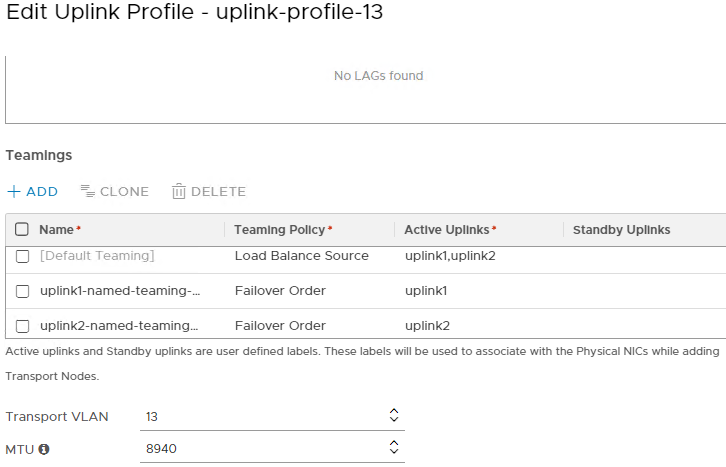
\includegraphics[width=1\textwidth]{imaxes/pruebaconcepto/UplinkPolicy13.png}
      \caption{Muestra la \textit{Uplink Policy} (\textit{uplink-profile-13}) configurada para la TZ \textit{sfo01-m01-dge-uplink-tz}. Se establece la VLAN 13 como Transport VLAN, utilizado para encapsular el tráfico saliente hacia la red física, y MTU de 8940 Bytes para los uplinks. Hay definidas tres \textit{Teaming Policies}, una por defecto (\textit{Default teaming}) que utiliza \textit{Load Balance Source} para hacer un mapeo uno a uno entre las interfaces de cada VM y uno de los \textit{uplinks} (todo el tráfico correspondiente a esa interfaz se envía y recibe por el mismo \textit{uplink}), y dos adicionales \textit{uplink1-named-teaming-policy} y \textit{uplink2-named-teaming-policy} que utilizan \textit{Failover Order} donde se establece un \textit{uplink} como activo por donde se transmite todo el tráfico y otros de reserva que se usan en caso de que el \textit{uplink} activo falle (en una de las políticas todo el tráfico se reenvía por \textit{uplink1} y en la otra por \textit{uplink2}).}
      \label{fig:Uplink-Policy-13-NSXT} 
    \end{figure}
    \FloatBarrier
    A los \textit{segments} \textit{VCF-edge-mgmt-cluster-segment-11} y \textit{VCF-edge-mgmt-cluster-segment-12} pertenecientes a la TZ \textit{sfo01-m01-dge-uplink-tz} se les asigna la \textit{Teaming Policy} \textit{uplink1-named-teaming-policy} y \textit{uplink2-named-teaming-policy} respectivamente. De esta forma se consigue que el tráfico que circula por cada uno de ellos solo utilice un único \textit{uplink}. 
    \begin{figure}[h]
      \centering
      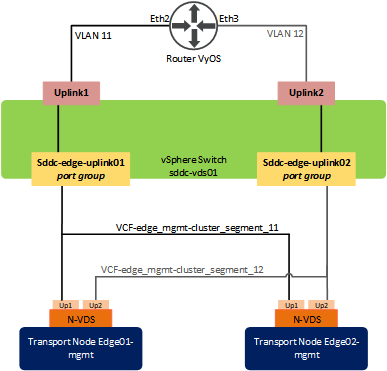
\includegraphics[width=0.6\textwidth]{imaxes/pruebaconcepto/UplinkDesign.png}
      \caption{Muestra la topología que forman las instancias de NSX-T Edge para generar la redundancia y alta disponibilidad en las rutas hacia la red externa para las aplicaciones cuya red está gestionada por VMware NSX-T, desde el punto de vista de VMware vSphere. Cada TN Edge posee dos interfaces \textit{uplink} que durante su configuración se mapea cada una con uno de los \textit{trunk port groups} de vSphere Switch. Las interfaces \textit{uplink} que se indican en la \textit{Teaming Policy} se refieren a las de la instancia de NSX-T Edge, no las de vSphere vSwitch, por lo tanto cada uno de los \textit{segments} utiliza solo uno de los \textit{uplinks} que combinado con la configuración de los \textit{port groups} de vSphere vSwitch establecen las rutas que se muestran en la imagen.}
      \label{fig:Uplink-Design-Edge-NSXT} 
    \end{figure}
    \FloatBarrier
    % Así, como cada TN de NSX-T Edge está anclado a dos \textit{trunk port groups} en vSphere Switch por donde se transmite el tráfico de estos dos \textit{segments} y cada uno de esos \textit{segments} transmite por un único \textit{uplink}, se consigue que estas rutas hacia la red externa sean redundantes y con alta disponibilidad para las aplicaciones cuya red está gestionada por VMware NSX-T.
    % Para la TZ de tipo VLAN \textit{sfo01-m01-dge-uplink-tz} se especifica la siguiente \textit{Uplink Policy}:
    % \begin{itemize}
    %   \item Nombre: \textit{uplink-profile-13}
    %   \item Transport VLAN: 13
    %   \item MTU: 8940
    %   \item Teaming Policy: se especifican tres, una por defecto y dos adicionales:
    %     \begin{itemize}
    %       \item \textit{Default teaming}: \textit{Load Balance Source}, hace un mapeo uno a uno entre cada interfaz virtual de cada VM y uno de los \textit{uplinks} del N-VDS, así todo el tráfico correspondiente a esa interfaz se envía y recibe por el mismo \textit{uplink}.
          
    %       \item \textit{uplink1-named-teaming-policy}: \textit{Failover Order}, se establece un \textit{uplink}, \textit{uplink1} en este caso, como activo que se utiliza para enviar todo el tráfico, y una lista de \textit{uplinks} ordenados que se utilizan en caso de que el primero no esté disponible, vacía para esta \textit{Teaming policy}.
    %       \item \textit{uplink2-named-teaming-policy}: \textit{Failover Order}, donde el \textit{uplink} activo es \textit{uplink2} y la lista de \textit{uplinks} de reserva está vacía.
    %     \end{itemize}
    % \end{itemize}
    % A los \textit{segments} de esta TZ, \textit{VCF-edge-mgmt-cluster-segment-11} y \textit{VCF-edge-mgmt-cluster-segment-12} se les asignan las \textit{Teaming Policy} \textit{uplink1-named-teaming-policy} y \textit{uplink2-named-teaming-policy} respectivamente. Con esta configuración el tráfico de cada \textit{segment} circula por una única NIC física del host ESXi. Esto, junto con la configuración \textit{Failover Order} establecida para los \textit{port groups} \textit{sddc-edge-uplink01} y \textit{sddc-edge-uplink02} en el vSphere vDS,se consigue que el tráfico de salida hacia la red física perteneciente a los componentes de VMware NSX-T y todas las aplicaciones cuya red gestiona VMware NSX-T, sea distribuído por dos redes distintas proporcionando redundancia y disponibilidad del servicio en caso de que ocurra una caída de alguna de las conexiones.
    %*****************%

    Esta encapsulación, tanto VLAN como Overlay, tiene lugar cuando los paquetes salen de la interfaz de una VM y entran en el N-VDS del TN. Para ello, cada TN tiene dispositivo llamado \textit{Tunnel End Point} (TEP) al que se le asigna una dirección IP utilizada para enviar y recibir el tráfico entre VMs que se encuentran en el mismo \textit{segment} pero se alojan en TNs situados en redes L2 diferentes\footnote{En el entorno desplegado todos los TN se encuentran dentro de la misma red física. Esto implica que no se genere tráfico con los TEPs ya que todas las TZs funcionan sobre un único dominio broadcast.}. Los TNs que son hosts ESXi obtienen su dirección TEP de un servidor DHCP\footnote{El servidor DHCP hace que se simplifique el proceso de configuración de un nuevo host ESXi ya que le asigna una dirección IP de forma automática.} mientras que los que son instancias de NSX-T Edge la dirección IP se asigna de forma manual. El TEP de cada TN tiene dos direcciones IP asignadas puesto que cada uno tiene dos interfaces de red, \textit{esxi-1} tiene las direcciones 172.16.254.10 y 172.16.254.11, \textit{esxi-2} tiene las direcciones 172.16.254.12 y 172.16.254.13, \textit{esxi-3} tiene las direcciones 172.16.254.14 y 172.16.254.15, \textit{esxi-4} tiene las direcciones 172.16.254.16 y 172.16.254.17, \textit{edge01-mgmt} tiene las direcciones 172.27.13.2 y 172.27.13.3, y \textit{edge02-mgmt} tiene las direcciones 172.27.13.4 y 172.27.13.5.
    
    Al crear un \textit{segment} dentro de una TZ, se configura un modo de replicación que indica como se retransmite el tráfico Broadcast, Multicast y Unknown Unicast propio del \textit{segment} cuando este tiene que viajar a un TN que está en una ubicación distinta en el medio físico. El modo de replicación que se utiliza en todos los \textit{segments} es \textit{Two-Tier Hierarchical Mode}. 
    \begin{figure}[h]
      \centering
      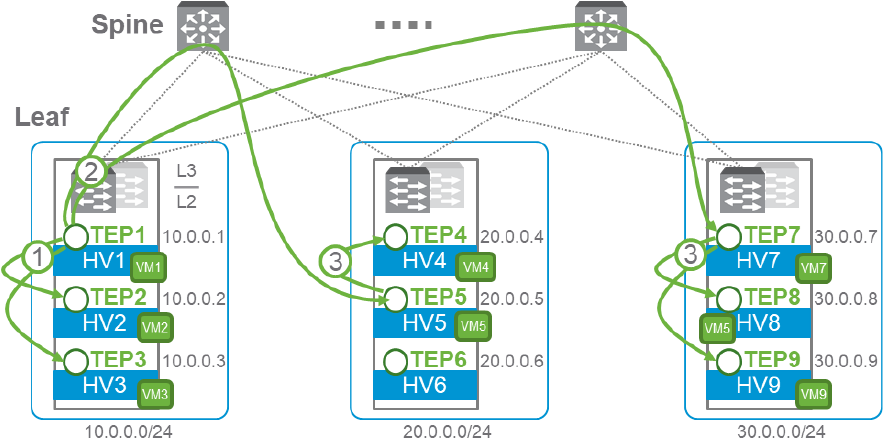
\includegraphics[width=0.6\textwidth]{imaxes/pruebaconcepto/Two-tier-ReplicationMode.png}
      \caption{Ejemplo de como funciona el modo de replicación \textit{Two-Tier Hierarchical}. (1) Cuando el TN HV1 envía tráfico BUM a la red primero lo hace a los TNs que están en su mismo dominio, (2) después envía una copia de ese tráfico a un único TN de cada dominio broadcast donde exista el \textit{segment} propietario del tráfico y, finalmente, (3) el TN de cada localización lo retransmite al resto de TNs de su dominio que lo requieran. De este modo se reduce el número de paquetes que el TN origen debe enviar a través de la red física.}
      \label{fig:Frame-Geneve-Segment-NSXT}
    \end{figure}
    \FloatBarrier
    % Este consiste en que cuando desde un TN se envía algún tipo de tráfico BUM de un \textit{segment} cuyos TNs están distribuídos en distintos puntos de la infraestructura física, el TEP del TN origen detecta que debe retransmitir el tráfico a una red externa, en la red externa se selecciona un TN que recibe el tráfico y lo reenvía al resto de TNs dentro del mismo dominio de red que deben recibir ese tráfico, así se reduce . El tráfico solo se enviará a los TN que contienen VMs que forman parte del \textit{segment} que lo genera. Es el componente NSX-T Controller quien se encarga de actualizar e indicar a los TNs toda la información para que esta comunicación sea correcta.
    
    El objetivo es crear nuevas subredes, es decir \textit{segments} que se expanden por los distintos TNs adheridos a la \textit{transport zone} correspondiente, y conectarlas a un router virtual para al final formar subredes distribuidas con servicios de red también	distribuidos y virtualizados, todo gestionado desde VMware NSX-T y sin tener que configurar la red física. Para completar esto, VMware NSX-T introduce routers virtuales que se encuentran embebidos y distribuídos dentro del hypervisor ESXi de cada TN y que proporcionan enrutamiento entre \textit{segments} y servicios de red distribuídos. Permiten definir un \textit{gateway} para cada \textit{segment} a través del cual las VMs conectadas pueden acceder a la red externa y los servicios de red. La herramienta VLC despliega para el \textit{management domain} un modelo de enrutamiento de doble capa (\textit{Two Tier Routing}) donde se utilizan dos routers virtuales, \textit{Tier-0} (\textit{mgmt-domain-tier0-gateway}) dedicado a gestionar el acceso a la red externa a través del router VyOS con conexiones redundantes, y \textit{Tier-1} (\textit{mgmt-domain-tier1-gateway})que gestiona el enrutamiento entre \textit{segments} y proporciona servicios de red a las VMs.

    \begin{figure}[h]
      \centering
      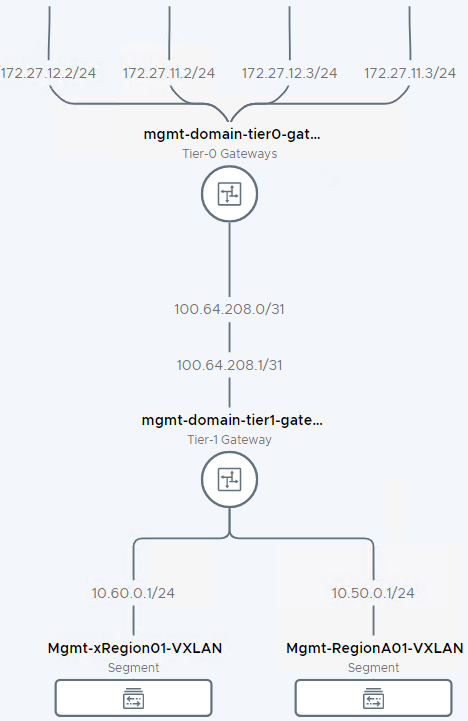
\includegraphics[width=0.5\textwidth]{imaxes/pruebaconcepto/topologiaTwoTierRouting.png}
      \caption{Muestra la topología del modelo de dos routers virtuales y los \textit{segments} a los que se conecta cada uno desde el punto de vista de NSX-T. El router de Tier-1 enruta el tráfico entre los \textit{segments} a los que está conectado y hacia el router de Tier-0 que se encarga de transmitir el tráfico hacia la red física.}
      \label{fig:Topology-TwoTier-Routing-NSXT}
    \end{figure}
    \FloatBarrier
    Un router router lógico está formado por dos componentes:
    \begin{itemize}
      
      \item \textbf{Distributed Router} (DR): que gestiona el enrutamiento y se a subredes a través de sus interfaces lógicas. Estas subredes pueden ser \textit{segments} u otro DR. A cada interfaz se le asigna una dirección MAC y una dirección IP que representa el \textit{gateway} de la subred. Este componente está distribuído en todos los TN, tanto hosts ESXi como instancias de NSX-T Edge manteniendo la misma configuración (interfaces,tablas de enrutamiento, etc.). Su función es redirigir el tráfico que recibe entre las interfaces que tiene disponibles, es decir, enruta el tráfico entre los diferentes \textit{segments} a los que está conectado el router virtual Tiene una interfaz llamada \textit{Internal transit Link} conectada a la red \textit{Internal Transit Network} que se utiliza para conectar todos los DR y SR de un \text{Tier} distribuídos en los TN.
      
      \item \textbf{Service Router} (SR): proporciona servicios de red de forma centralizada (NAT, DHCP, Load Balancer, VPN, Gateway Firewall y Bridging L2) y proporciona acceso a la red externa. Este componente no está distribuído entre los diferentes TN, solo se se encuentra distribuido en las instancias de NSX-T Edge. Los servicios que proporciona solo se entregan a los recursos cuya red está gestionada por VMware NSX-T. Posee la interfaz \text{Internal Transit Link} para comunicarse con el resto de DR y SR pertenecientes al mismo \text{Tier}, dos interfaces \textit{External Interface} que se conectan a los \text{segments} que dan acceso a la red externa \footnote{La \textit{External Interface} solo existe en \textit{Tier-0} ya que es el router que se comunica con el dispositivo físico.}, la interfaz \textit{Router Link}\footnote{Router Link Network utiliza por defecto la subred 100.64.0.0/16.} que conecta el SR de \textit{Tier-0} con el de \textit{Tier-1}, y la interfaz \textit{Internal transit} que se habilita cuando se activa la opción \textit{Inter SR iBGP}\footnote{Inter SR iBGP Network utiliza por defecto la subred 169.254.0.0/24.} y que comunica los SR de las dos instancias de NSX-T Edge.
    \end{itemize}

    \begin{figure}[h]
      \centering
      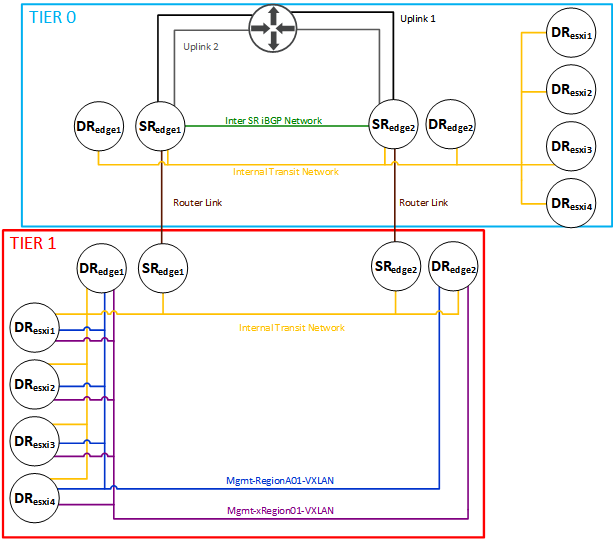
\includegraphics[width=0.8\textwidth]{imaxes/pruebaconcepto/EstructuraInternaTiers.png}
      \caption{Muestra los componentes internos de cada router virtual y como estos están distribuidos por todos los TNs. El router \textit{mgmt-domain-tier0-gateway} tiene el componente SR distribuído en dos TN que son las instancias de NSX-T Edge, y el componente DR distribuido en todos los TNs. El SR situado en \textit{edge01-mgmt} está conectado al \textit{segment} \textit{VCF-edge\_mgmt-edge-cluster-segment-11} y usa la dirección IP 172.27.11.2, y otra interfaz conectada al \textit{segment} \textit{VCF-edge\_mgmt-edge-cluster-segment-12} donde usa la IP 172.27.12.2, mientras que el SR de \textit{Tier-0} situado en \textit{edge02-mgmt} se conecta a los mismos \textit{segments} pero usando las direcciones 172.27.11.3 y 172.27.12.3 respectivamente. El router \textit{mgmt-domain-tier1-gateway} tiene el componente SR distribuido en las dos instancias de NSX-T Edge y el componente DR distribuido por en todos los TNs. Ambos SR están conectados con los SR de \textit{Tier-0} para transmitir el tráfico hacia la red física. Los DR de \textit{Tier-1} están conectados a los \textit{segments} \textit{Mgmt-RegionA01-VXLAN} y \textit{Mgmt-xRegion01-VXLAN} para proporcionar enrutamiento y servicios a las VMs situadas en ellos.}
      \label{fig:estructura-interna-TwoTier-Routing-NSXT}
    \end{figure}
    \FloatBarrier
    
    La razón de tener dos capas de enrutamiento se debe a la configuración del router \textit{mgmt-domain-tier0-gateway}. En este router se utiliza BGP para comunicarse con el router físico a través de las \textit{external interfaces} (se establece 65003 como \textit{autonomous system} local)\footnote{El uso de BGP simplifica la configuración de nuevas rutas cuando se añaden componentes al entorno, y que no se pierda la conectividad en caso de caída de alguna de las interfaces. Este protocolo también se configura en las interfaces del router Vyos}, la opción \textit{Inter SR iBGP} establecer una comunicación mediante BGP entre las instancias distribuídas del componente SR de \textit{Tier-0} para que se pueda seguir transmitiendo el tráfico en caso de que alguna de las interfaces de una instancia de NSX-T Edge esté fuera de servicio, se activa el protocolo ECMP para balancear el tráfico hacia la red física entre los caminos disponibles ya que en conjunto, en el router de \textit{Tier-0} existen cuatro rutas posibles para alcanzar el router VyOS. Un aspecto importante es la configuración de la disponibilidad de un router virtual ya que determina el modo en el que se va a ejecutar. En el router de \textit{Tier-0} se selecciona el modo \textit{active-active} el cual implica que las dos instancias de SR funcionan ambas de forma activa, es decir, el tráfico que reciba cada una será encaminado por una subred diferente proporcionando así mayor ancho de banda, mayor disponibilidad y mayor escalabilidad. Esto esto último no es compatible con servicios de red centralizados, por ello es necesario desplegar al menos un router lógico de \textit{Tier-1} (\textit{mgmt-domain-tier1-gateway}) configurado con el modo \textit{active-stanby} el cual solo se utiliza una de las dos instancias del SR de \textit{Tier-1} por lo tanto el tráfico dirigido a este router siempre será recogido en un único punto. Así, en el router \textit{mgmt-domain-tier1-gateway} es donde se pueden desplegar servicios de red como NAT, Load Blancing, DNS y VPN, para los \textit{segments} que están conectados.
    % Las interfaces de cada router lógico son de los siguientes tipos:
    
    % \begin{itemize}
    %   \item \textit{External Interface}: se refiere a las interfaces que conectan con el dispositivo de la red física, normalmente un router.
    %   \item \textit{Internal Transit Link}: está interfaz conecta a todos los DR de \textit{Tier-0} distribuídos en cada TN con los SR formando una única red.
    %   \item \textit{RouterLink Interface}: interfaz que conecta un router lógico de \textit{Tier-1} con uno de \textit{Tier-0} a través de una subred generada por defecto (100.64.0.0/16).
    % \end{itemize}
    
    % Los routers lógicos creados para el \textit{management domain} en el entorno tienen la siguiente configuración:
    
    % \begin{itemize}
    %   \item \textbf{mgmt-domain-tier0-gateway}: su función consiste en proporcionar acceso a la red física.
    %     \begin{itemize}
    %       \item \textit{External Interfaces}\footnote{Estas direcciones corresponden a las interfaces de los TN NSX-T Edge que conectan con las interfaces Uplink sobre dos \textit{segments} de tipo VLAN.}: Dos que se conectan al \textit{segment} \textit{VCF-edge\_mgmt-edge-cluster-segment-11} (172.27.11.2 y 172.27.11.3) y dos que se conectan al \textit{segment} \textit{VCF-edge\_mgmt-edge-cluster-segment-12} (172.27.12.2 y 172.27.12.3).
    %       \item \textit{Internal Transit Link}: Usa la subred 169.254.0.0/24.
    %       \item \textit{RouterLink Interface}: Tiene la dirección 100.64.192.0/31.
    %       \item Configuración: se 
    %       \item Configuración HA: determina el modo en el que se va a ejecutar el router de \textit{Tier-0}. En este caso se selecciona el modo \textit{active-active} el cual implica que las instancias de SR (una en cada nodo NSX-T Edge) funcionan ambas de forma activa, el tráfico que reciba cada una será encaminado por una subred diferente. Es por esto que el router lógico de \textit{Tier-0} no puede ofrecer servicios centralizados.
    %     \end{itemize}
    
    %   \item \textbf{mgmt-domain-tier1-gateway}: router de \textit{Tier-1} dedicado a gestionar el enrutamiento de las VMs de aplcaciones no dedicadas a la administración del SDDC. 
    %   \begin{itemize}
    %     \item \textit{Internal Transit Link}: Usa la subred 164.254.0.0/24.
    %     \item \textit{RouterLink Interface}: Tiene la dirección 100.64.192.1/31.
    %     \item \textit{Segment Interfaces}: conectado al \textit{segment} \textit{mgmt-Region01A-VXLAN} con la dirección IP 10.50.0.1, y al \textit{segment} \textit{mgmt-xRegion01-VXLAN} con la dirección IP 10.60.0.1.
    %     \item Configuración HA: determina el modo en el que se va a ejecutar el router de \textit{Tier-1}. En este caso se selecciona el modo \textit{active-stanby} el cual solo utiliza una de las dos instancias del SR de \textit{Tier-1} (cada una en un nodo de NSX-T Edge) por lo tanto el tráfico que reciba solo será encaminado por un único punto. Esto permite activar servicios centralizados, por lo tanto será \textit{mgmt-domain-tier1-gateway} y no \textit{mgmt-domain-tier0-gateway} el encargado de proporcionarlos.
    %   \end{itemize}
    % \end{itemize}
    
    % Así como el componente DR de los routers de \textit{Tier-0} y de \textit{Tier-1} están distribuídos por todos los TNs (incluídas las instancias de NSX-T Edge), el componente SR solo se encuentra en las VMs de NSX-T Edge por lo tanto son estas VMs las que proporcionan los servicios centralizados de SR y acceso a la red externa del entorno. Además, para que los componentes lógicos tengan acceso a los \textit{segments} descritos, las instancias de NSX-T Edge están conectadas a dos TZs:
    % \begin{itemize}
      
    %   \item \textit{mgmt-domain-m01-overlay-tz}: esta TZ proporciona a las VMs del entorno a los servicios de los routers de \textit{Tier-0} y de \textit{Tier-1} y también permite que esos routers lógicos tengan acceso a los \textit{segments} donde se encuentran esas VMs. Se utiliza el tipo Overlay para que se puedan comunicar TNs que se encuentran en distintas redes físicas sin que la configuración de la red física sea compleja.
      
    %   \item \textit{sfo01-m01-dge-uplink-tz}: esta TZ se utiliza para conectarse a la red física a través de un router físico. Se utiliza el tipo VLAN para encapsular el tráfico saliente hacia al router físico y porque las VLANs usadas en los \textit{segments} dentro de esta TZ se configuran también en la infraestructura física, por lo tanto no hace falta crear una capa física virtual con Overlay.
    % \end{itemize}
    
    % Para gestionar las conexiones de cada TN, tanto para los nodos NSX-T Edge como para los hosts ESXi, VMware NSX-T introduce el componente llamado \textbf{NSX-T Virtual Distributed Switch} (N-VDS). Cada TN del entorno posee un N-VDS, este elemento conecta sus interfaces a los \textit{segments} que se configuran en cada TN y establece un mapeo con las interfaces \textit{uplink} que se utilizan para dirigir el tráfico de cada TZ hacia el exterior del TN. En el caso de las instancias de NSX-T Edge, los dos \textit{uplinks} están mapeados con las NICs físicas de cada host ESXi a través de los dos \textit{distributed port groups} de vSphere vDS (\textit{sddc-edge-uplink01} y \textit{sddc-edge-uplink02}) a los que están ancladas ambas VMs, es decir, un \textit{uplink} está mapeado con una NIC física del host ESXi. 
    % En las TZ de tipo VLAN, se utilizan plantillas \textit{Uplink Policy} para indicar como debe el N-VDS tratar el tráfico de la \textit{transport zone} a la que se asigna. En cada \textit{Uplink Policy} se especifican varias \textit{Teaming Policy}, el identificador VLAN que debe usar el N-VDS cuando tiene que enviar el tráfico fuera del TN y el MTU de los \textit{uplinks}. Una \textit{Teaming Policy} indica como el N-VDS utiliza los \textit{uplinks} para conseguir conexiones redundantes y balanceo de la carga, en una \textit{Uplink Policy} se especifica una \textit{Teaming Policy} por defecto y otras adicionales.
    % Para la TZ de tipo VLAN \textit{sfo01-m01-dge-uplink-tz} se especifica la siguiente \textit{Uplink Policy}:
    % \begin{itemize}
    %   \item Nombre: \textit{uplink-profile-13}
    %   \item Transport VLAN: 13
    %   \item MTU: 8940
    %   \item Teaming Policy: se especifican tres, una por defecto y dos adicionales:
    %     \begin{itemize}
    %       \item \textit{Default teaming}: \textit{Load Balance Source}, hace un mapeo uno a uno entre cada interfaz virtual de cada VM y uno de los \textit{uplinks} del N-VDS, así todo el tráfico correspondiente a esa interfaz se envía y recibe por el mismo \textit{uplink}.
          
    %       \item \textit{uplink1-named-teaming-policy}: \textit{Failover Order}, se establece un \textit{uplink}, \textit{uplink1} en este caso, como activo que se utiliza para enviar todo el tráfico, y una lista de \textit{uplinks} ordenados que se utilizan en caso de que el primero no esté disponible, vacía para esta \textit{Teaming policy}.
    %       \item \textit{uplink2-named-teaming-policy}: \textit{Failover Order}, donde el \textit{uplink} activo es \textit{uplink2} y la lista de \textit{uplinks} de reserva está vacía.
    %     \end{itemize}
    % \end{itemize}
    % A los \textit{segments} de esta TZ, \textit{VCF-edge-mgmt-cluster-segment-11} y \textit{VCF-edge-mgmt-cluster-segment-12} se les asignan las \textit{Teaming Policy} \textit{uplink1-named-teaming-policy} y \textit{uplink2-named-teaming-policy} respectivamente. Con esta configuración el tráfico de cada \textit{segment} circula por una única NIC física del host ESXi. Esto, junto con la configuración \textit{Failover Order} establecida para los \textit{port groups} \textit{sddc-edge-uplink01} y \textit{sddc-edge-uplink02} en el vSphere vDS,se consigue que el tráfico de salida hacia la red física perteneciente a los componentes de VMware NSX-T y todas las aplicaciones cuya red gestiona VMware NSX-T, sea distribuído por dos redes distintas proporcionando redundancia y disponibilidad del servicio en caso de que ocurra una caída de alguna de las conexiones.
    
    
    
    % Estas conexiones están gestionadas por un N-VDS dentro de cada instancia. Este switch lógico utiliza tres interfaces que se conectan a las diferentes redes lógicas. Para aquellas redes lógicas que requieren salida al medio físico ya sea para comunicarse con otros TN o para acceder a la red externa, el N-VDS utiliza finalmente el switch VDS de VMware vSphere que conecta con las interfaces físicas del host ESXi donde corre la instancia de NSX-T Edge.
    
    % la utilizan tres interfaces para  Estas interfaces son \textit{eth0} que se dedica a la red \textit{Management}, \textit{fp-eth0} y \textit{fp-eth1} que ambas se dedican a la conexión con cada uno de los \textit{segments} Uplink. 
    
    
    % *********************************************
    
    %%%%%%%%
    % Se recomienda que la red física siga una topología de tipo \textit{Leaf-Spine} donde existen swithces que se conectan a los hosts (\textit{leaf switches}), que a su vez se conectan a otra capa de switches (\textit{spine switches}) que finalmente conecta con la red principal del SDDC. Este tipo de topología permite medir mejor su rendimiento y facilita la escalabilidad de la infraestructura. En caso de existir varias AZ, debe existir una red física entre ellas cuya capa 3 funcione con enrutamiento dinámico para automatizar la resolución de problemas en caso de caída de alguna de las conexiones.
    %%%%%%%%%
    
    % \iffalse
    % La información sobre VTEP existentes, la relación entre direcciones MAC de máquinas virtuales y dirección IP de VTEP, y relación entre direcciones MAC de máquinas virtuales y su IP, la poseen las instancias de NSX Controller en tres tablas: 
    %     \begin{itemize}
    %         \item \textit{VTEP Table}, relación entre un VTEP y la VXLAN que tiene acceso: VNI (ID del segmento), IP (dirección IP del VTEP), Segment (dirección IP del segmento), MAC (dirección MAC de la NIC física donde está configurado el VTEP).
    %         \item \textit{MAC Table}, relación entre la dirección MAC de una máquina virtual y el VTEP que le da acceso: VNI (ID del segmento), MAC (dirección MAC de la máquina virtual accesible por la VTEP-IP), VTEP-IP (dirección IP del VTEP que da acceso a la máquina virtual de la MAC indicada).
    %         \item \textit{ARP Table}, relación entre la dirección MAC y la dirección IP de una máquina virtual: VNI (ID del segmento), IP (dirección IP de la máquina virtual), MAC (dirección MAC de la máquina virtual).
    %     \end{itemize}
    % Estas tablas permiten reducir la cantidad de tráfico en la red ya que las máquinas virtuales y dispositivos de enrutamiento ya no requieren enviar tráfico Broadcast para obtenerla.
    % La comunicación directa entre máquinas virtuales situadas en distintos hosts ESXi se realiza con tráfico Unicast entre sus respectivos VTEP, pero una máquina virtual también puede enviar tráfico dirigido a todas las máquinas virtuales que pertenecen a su mismo Logical Switch, es decir, a las máquinas de la misma \textit{trasnport zone}, pero pueden situarse en segmentos de red físicos distintos. Este tipo de tráfico puede ser Multicast, Unknown Unicast y Broadcast (BUM), y en VMware NSX se puede gestionar con tres modos de replicación distintos\footnote{Al configurar un Logical Switch se elige uno de los modos.}, modo Multicast, modo Unicast y modo Híbrido.
    %     \begin{itemize}
    %         \item \textbf{Modo Multicast}: requiere que en la red física se haya configurado una IP multicast para cada VXLAN (es decir, Logical Switch), y el protocolo IGMP Snooping en los switches físicos para crear grupos multicast y que el tráfico sea más eficiente, esto habilita multicast entre los VTEP de la misma subred que el emisor. Para transmitir este tráfico a VTEPs situados en otros segmentos de red, se debe configurar el protocolo PIM para poder enrutarlo con los dispositivos de capa 3 físicos. Esta configuración no permite desacoplar la red lógica de la red física.\\
    %         Se puede establecer un grupo multicast por cada VXLAN, esto implica que un host solo recibirá tráfico si tiene al menos una máquina virtual en el grupo, pero requiere configurar muchos grupos. Otra opción es crear un grupo multicast para todas las VXLAN, se necesitan menos direcciones IP pero se genera más tráfico en la red.
    %     \begin{figure}[h!]
    %     \centering
    %     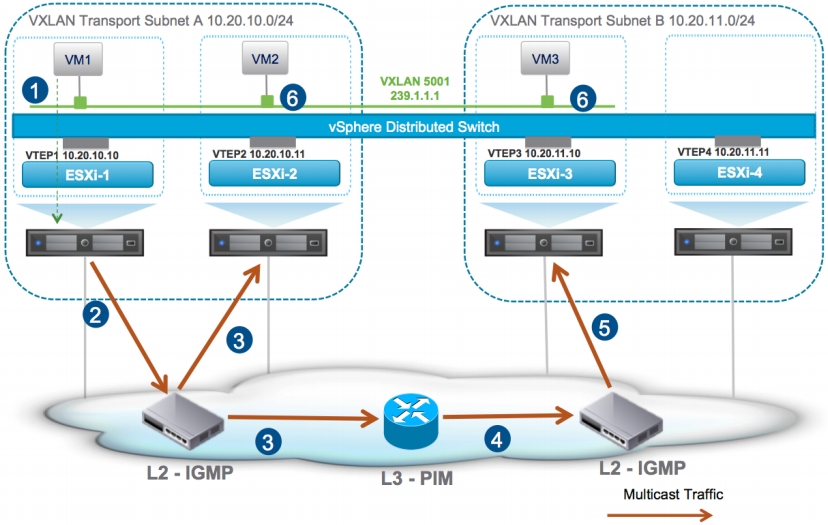
\includegraphics[width=0.5\textwidth]{imaxes/conceptosPrevios/MulticastSeqBUM.png}  \caption{Replicación del tráfico BUM en el modo Multicast}
    %     \label{fig:modoMulticast}
    %     \end{figure}
    %     \FloatBarrier
    %         \item \textbf{Modo Unicast}: no requiere ninguna configuración específica en la capa física y está gestionado por VMware NSX. Se crea un grupo con los VTEP situados en el mismo segmento de red, dentro de cada grupo se selecciona un host ESXi para el rol de \textit{Unicast Tunnel End Point} (UTEP), encargado de recibir el tráfico BUM que procede de otros segmentos de red para reenviarlo por su segmento pero solo a los hosts con al menos una máquina virtual. El host ESXi emisor utiliza la tabla VTEP para comprobar que VTEPs están situados en una VXLAN y así poder dirigir el tráfico BUM correspondiente.\\
    %         Este modo es útil en entornos pequeños donde no hay mucho tráfico y cada segmento de red tiene pocos VTEP.
    %     \begin{figure}[h!]
    %     \centering
    %     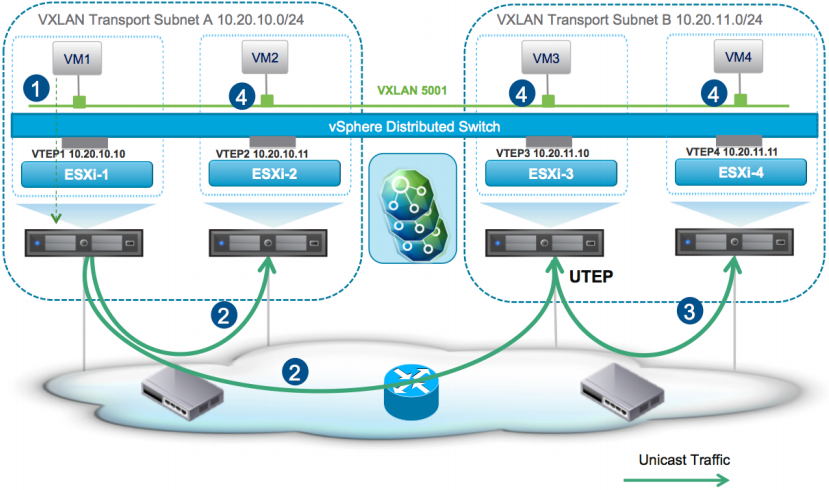
\includegraphics[width=0.5\textwidth]{imaxes/conceptosPrevios/UnicastMode.png}
    %     \caption{Replicación del tráfico BUM en el modo Unicast}
    %     \label{fig:modoUnicast}
    %     \end{figure}
    %     \FloatBarrier
    %         \item \textbf{Modo Híbrido}: combina el modo Unicast y el modo Multicast. El tráfico dirigido a las máquinas virtuales situadas en el mismo segmento de red se transmite usando Multicast, por lo que se requiere tener el protocolo IGMP configurado en los dispositivos físicos de capa 2, se recomienda establecer una dirección Multicast por cada VXLAN. El tráfico se replica a los hosts ESXi que forman parte del grupo. Cuando el tráfico va dirigido a máquinas virtuales situadas en hosts en distinto segmento de red, se transmite utilizando Unicast, como en ese modo, se forma un grupo con los hosts de cada segmento y de cada grupo se elige un host con el rol de \textit{Multicast Tunnel EndPoint} (MTEP). Así, el host que origina el tráfico BUM lo transmite al MTEP correspondiente, el cual se encarga de replicar ese tráfico por su segmento de red. La replicación del tráfico entre segmentos es gestionada por las instancias de NSX Controller.\\
    %         Este modo de replicación permite desplegar NSX en entornos grandes gracias a que el tráfico Multicast y Unicast se pueden escalar facilmente, el primero se reduce a cada segmento de red y la transmisión del segundo en la capa 3 está gestionado por VMware NSX sin necesidad de configurar los dispositivos físicos.
    %     \begin{figure}[h!]
    %         \centering
    %         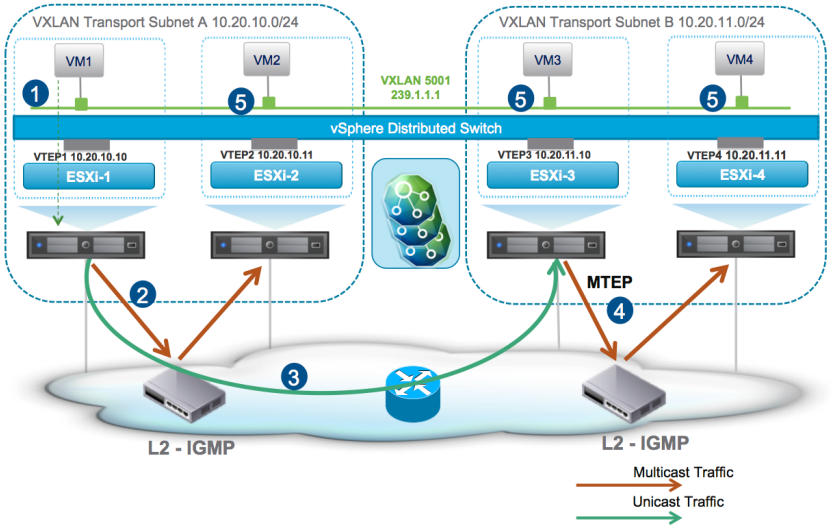
\includegraphics[width=0.5\textwidth]{imaxes/conceptosPrevios/hibrydMode.png}
    %         \caption{Replicación del tráfico BUM en el modo Híbrido}
    %         \label{fig:modoHibrido}
    %     \end{figure}
    %     \FloatBarrier
    %     \end{itemize}
    
    %  El enrutamiento del tráfico está gestionado por dos componentes Distributed Logical Router (DLR) y NSX Edge Services Gateway (ESG). Un mismo DLR se extiende por varios hosts ESXi para enrutar el tráfico entre VXLANs, también mantiene una conexión con las instancias de ESG para transmitir el tráfico que se dirige a redes externas, esa conexión se denomina \textit{transit network} y está getionada por un Logical Switch. Cada DLR tiene su propio Logical Router Control para intercambiar las rutas disponibles con las instancias de ESG, posteriormente, son las instancias de NSX Controller las que transmiten esta información al DLR distribuido en los hosts ESXi. Las interfaces lógicas del DLR conectan con cada Logical Switch, cada interfaz tiene una dirección IP que representa el \textit{gateway} del segmento de red al que esté conectada [Fig. \ref{fig:logicalRoutingCompo} y \ref{fig:redLogicaOne}]. Estos dispositivos utilizan enrutamiento dinámico (protocolos OSPF o BGP).
     
    %  \begin{figure}[h!]
    %   \centering
    %   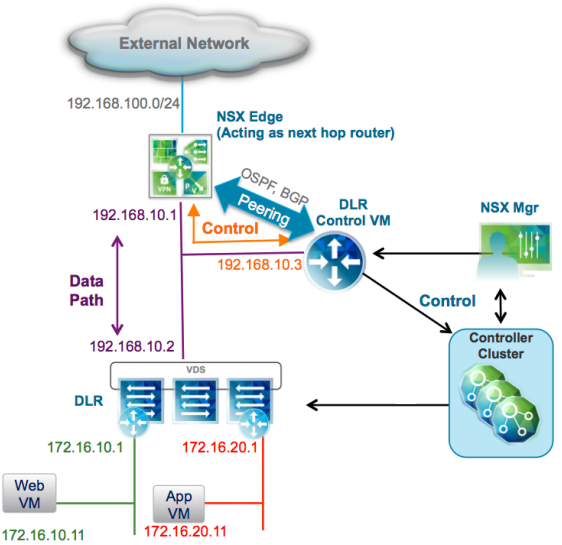
\includegraphics[width=0.4\textwidth]{imaxes/conceptosPrevios/LogicalRoutingComponents.png}
    %   \caption{Componentes de la red virtual que intervienen en el enrutamiento del tráfico.}
    %   \label{fig:logicalRoutingCompo}
    % \end{figure}
    % \FloatBarrier
    
    % \begin{figure}[h!]
    %   \centering
    %   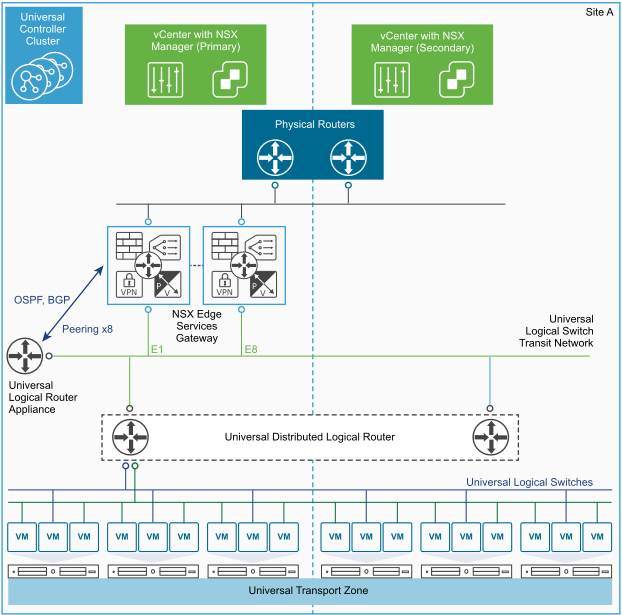
\includegraphics[width=0.5\textwidth]{imaxes/conceptosPrevios/redlogCF.png}
    %   \caption{Red lógica formada en un SDDC con dos clusters.}
    %   \label{fig:redLogicaOne}
    % \end{figure}
    % \FloatBarrier
     
    %  En el SDDC deben existir, al menos, dos intancias de ESG aunque se pueden desplegar hasta 8 instancias. En el modelo consolidado se debe tener un único UDLR para que las rutas entre hosts ESXi sean más cortas, debe existir un Logical Switch que forme la \textit{transit zone}. En el modelo estándar debe existir un UDLR extendido por todos los \textit{Management Cluster} (si hay varias \textit{Regions}), un UDLR extendido por el \textit{Shared Edge and Compute Cluster} y el resto de \textit{Compute Clusters} en cada \textit{Region}, y un DLR extendido por todos los clusters de una misma región.En el modelo estándar existen dos tipos de \textit{transit zones}, una entre el UDLR que atraviesa todas las \textit{Regions} y cada instancia de ESG, y otra que conecta el DLR propio de cada \textit{Region} y sus instancias de ESG. 
    % \\
    % Algunos componentes de VMware Cloud Foundation se deben desplegar en una VXLAN dedicada para proporcionar recuperación ante fallos en caso de que parte del SDDC deje de funcionar. Entre otros componentes (solo vamos a tratar aquellos que son obligatorios), VMware vRealize Log Insight se debe desplegar en una red de este tipo, llamada \textit{Application Virtual Network} (AVN). En entornos con varias \textit{Regions} se crea una \textit{transport zone} que se extiende por todo el SDDC y una \textit{transport zone} adicional en cada \textit{Region}, la primera proporciona recuperación ante fallos a través de todo el SDDC a los componentes que lo requieran, y la segunda solo a través de una \textit{Region}, sin necesidad de reconfigurar direcciones IP o DNS. VMware vRealize Log Insight se debe desplegar en una VXLAN por cada \textit{Region}.
    % \\
    % El acceso a una AVN se realiza a través de las instancias de ESG desplegadas en el entorno, estas se conectan a un UDLR que gestiona el tráfico de la s máquinas virtuales que tiene conectadas. El enrutamiento debe ser dinámico con BGP y las instancias de ESG proporcionan protegen y balacean la carga de trabajo con los servicios de VMware NSX Firewall y Load Balancing [Fig. \ref{fig:avnConsolidated}].\\
    % **VERIFICAR LO DEL LOAD BALANCING en el despliegue. ¿solo para las que son cross-region o tambien en las de una sola region**\\
    % \begin{figure}[h!]
    %   \centering
    %   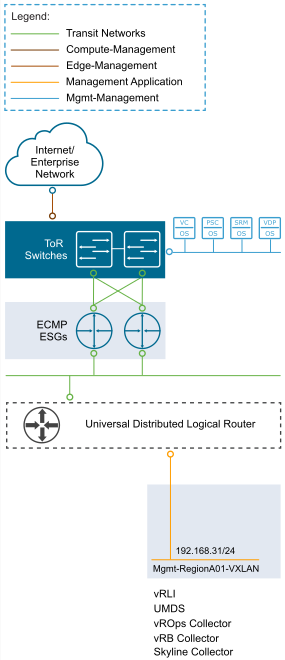
\includegraphics[width=0.25\textwidth]{imaxes/conceptosPrevios/AVNConsolidated.png}
    %   \caption{AVN en el modelo consolidado}
    %   \label{fig:avnConsolidated}
    % \end{figure}
    % \FloatBarrier
    
    % Este utiliza los componentes vCenter Server, NSX Manager, NSX Controllers y NSX Logical Switch para establecer comunicaciones y aislar los distintos tipos de tráfico [Fig. \ref{fig:planosNSX}]. Estos componentes \underline{actúan en diferentes planos} de la red:
    
    
    
    % \begin{itemize}
    %     \item \textbf{Plano de Datos}: esta capa gestiona la transmisión del tráfico entre los componentes del SDDC. En este plano actúan NSX Logical Switches segregando los tipos de datos, y el enrutamiento y firewall distribuído de NSX. Se transmite a través de una red física dedicada al transporte.
    %     \item \textbf{Plano de Control}: aquí se gestionan los mensajes de control que se usan para la configuración de los dispositivos de NSX como switches, routers y firewalls en cada host ESXi. Se distribuye en redes físicas de forma segura usando VLANs para aislarlo del plano de datos.
    %     \item \textbf{Plano de gestión}: aquí se gestiona el tráfico dedicado a la administración de los recursos como puede ser la creación y eliminación de máquinas virtuales. Está controlado por vCenter Server y NSX Manager.
    % \end{itemize}
    % \begin{figure}[h!]
    %   \centering
    %   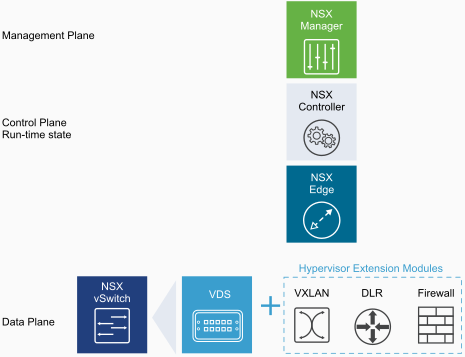
\includegraphics[width=0.65\textwidth]{imaxes/conceptosPrevios/planosNSX.png}
    %   \caption{Como se estructuran las componentes de VMware NSX for vSphere}
    %   \label{fig:planosNSX}
    % \end{figure}
    % \FloatBarrier
    
    %\fi
    
    % \iffalse
    % \subsubsection{Almacenamiento Virtual}
    % VMware vSAN forma único \textit{datastore} con todos los dispositivos de almacenamiento que se encuentran en la infraestructura permitiendo establecer políticas y gestionar esos recursos de forma más simple. Para que funcione correctamente es necesario \underline{configurar una red para VMware vSAN} teniendo en cuenta los siguientes aspectos:
    % \begin{itemize}
    %     \item El uso de vSpehere Distributed Switches genera mejor rendimiento.
    %     \item Se recomienda el uso de paquetes tipo \textit{jumbo frames}.
    %     \item Asignar una VLAN al tráfico de cada cluster de VMware vSAN.
    %     \item Si se implementa en un SDDC con dos localizaciones, es necesario establecer un host \textit{witness}.
    % \end{itemize}
    % Al establecer el tamaño y capacidad de este cluster hay que tener en cuenta que cuantos más hosts ESXi se incluyan, mayor tolerancia a fallos se tendrá y mejor se podrán repartir los grupos de discos entre todos los hosts. Debe haber un balance entre el hardware y la capacidad requerida.
    
    
    % \fi
    \end{subsection}
    
    \begin{subsection}{Operaciones de la Arquitectura}
    El entorno ya está configurado para funcionar como un SDDC, a partir de este punto ya no es necesario realizar ninguna modificación en la infraestructura física ya que todas las tareas que se deben realizar están dentro del alcance de los componentes de VMware Cloud Foundation. Para finalizar la construcción del SDDC y habilitar un servicio donde los usuarios puedan aprovisionar recursos bajo demanda, se instalarán sobre el entorno desplegado las aplicaciones Workspace ONE Access \footnote{VMware vRealize Identity Manager} (WSA) y VMware vRealize Automation (vRA). La primera permite al administrador conectar con el servidor de usuarios Active Directory y gestionarlos para proveer un servicio de autenticación centralizado a múltiples aplicaciones como VMware vRealize Automation. La segunda aplicación permite a los usuarios aprovisionar recursos de forma automatizada desde un catálogo de recursos. VMware vRealize Suite Licfecycle Manager (vRSLCM) es el componente que permite administrar vRA y WSA, su instalación y actualizaciones, las contraseñas de administrador y sus certificados, para ello necesita comunicarse con VMware vCenter Server. Se desplegará una instancia de cada componente en el \textit{management domain} creado anteriormente y estarán conectadas al \textit{segment}/subred \textit{Mgmt-xRegion01-VXLAN}.
    
    % \begin{subsubsection}{vRealize Suite Lifecycle Manager}
        
    % \end{subsubsection}
    \begin{subsubsection}{Workspace One Access}
        Los usuarios que necesiten acceder a vRA deben estar registrados en el directorio de Workspace One Access. Este componente centraliza el acceso de todos los productos de VMware vRealize. Cuando se despliega se debe configurar un Active Directory que en el caso del entorno está situado en la VM con Windows Server 2016. Dentro del Active Directory existen grupos de seguridad y perfiles de usuario, un perfil de usuario contiene información como nombre, apellidos, dirección e-mail, nombre de usuario y contraseña\footnote{Se pueden configurar más campos pero los que se describen son los obligatorios a la hora de crear un usuario.}, y este puede formar parte de varios grupos de seguridad. Una vez configurado, cada aplicación se conectará a WSA y se podrán asignar roles para los grupos de seguridad y usuarios estableciendo así un nivel de acceso. Además, cada usuario registrado tendrá disponible un catálogo de aplicaciones en el portal de WSA cuyo administrador establecerá que aplicaciones están habilitadas para cada usuario o grupo, eso sí, para que el usuario pueda acceder a ella previamente se debe establecer un rol para ese usuario dentro de la aplicación.

        %*****USUARIOS QUE HAY EN EL ENTORNO Y EL ACCESO A CADA APLICACIÓN*******%
        \begin{figure}[h]
            \centering
            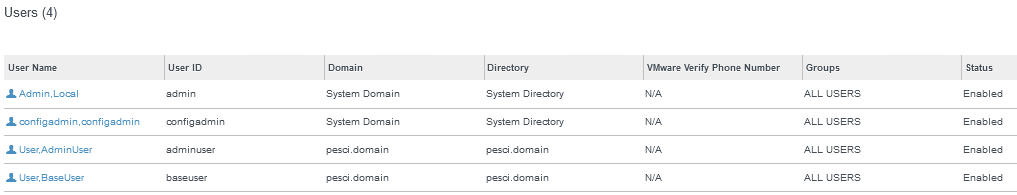
\includegraphics[width=0.4\textwidth]{imaxes/vRealize_pruebaconcepto/usuariosDefinidos.png}
            \caption{Muestra los usuarios definidos en el Active Directory sincronizados en Workspace One Access.}
            \label{fig:users-defined-AD}
        \end{figure}
        \FloatBarrier
        En la Figura \ref{fig:users-defined-AD} se muestran los dos usuarios definidos en el Active Directory y dos usuarios que se corresponden a los perfiles de administración de WSA, no se utilizarán grupos de seguridad para reducir la complejidad pero su configuración en las aplicaciones de VMware es igual que para los perfiles de usuario. En un entorno real existen usuarios que controlan a otros usuarios y establecen su nivel de acceso, a parte de los perfiles de administrador de cada aplicación. Para el entorno se define el perfil \textit{adminuser} que será el encargado de gestionar el acceso de dos usuarios (\textit{baseuser1} y \textit{baseuser2}) que serán los que consuman a las aplicaciones desplegadas (vRSLCM y vRA). El primero tendrá acceso y permisos de edición en las aplicaciones vRSLCM y vRA, mientras que los dos usuarios base solo podrán acceder a vRA y dentro de este el usuario admin definirá que servicios están habilitados para cada uno.

        %************************************************************************%

    \end{subsubsection}

    \begin{subsubsection}{VMware vRealize Automation}
        El punto a través del cual los usuarios pueden aprovisionar sus recursos es vRealize Automation. Este producto provee el servicio cloud. 
        \begin{figure}[h]
            \centering
            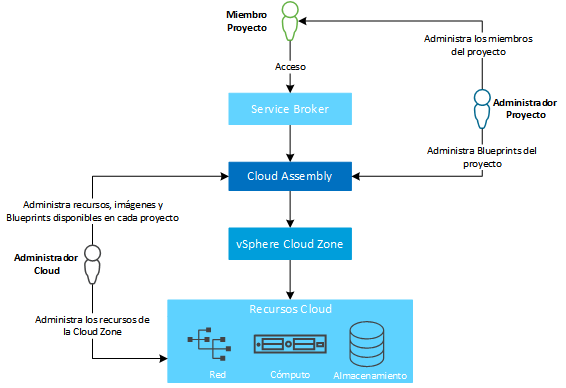
\includegraphics[width=0.8\textwidth]{imaxes/vRealize_pruebaconcepto/ComponentesVRA.png}
            \caption{Componentes de VMware vRealize Automation y tareas que realiza cada rol de usuario.}
            \label{fig:users-defined-AD}
        \end{figure}
        \FloatBarrier
        Internamente vRA se divide en varios servicios que permiten gestionar los diferentes aspectos de la cloud. Para centrarse en los objetivos de este proyecto solo se hace referencia a dos de esos servicios, el primero es Cloud Assembly el cual permite administrar la infraestructura disponible controlar el uso que se hace de esos recursos, y el segundo es Service Broker, utilizado por los usuarios para aprovisionar los recursos desde un catálogo de plantillas. La obtención de los recursos por parte del usuario se hace desplegando una serie de plantillas llamadas Blueprints diseñadas previamente, en donde se define un conjunto de VMs y recursos de red y de almacenamiento incluyendo otros aspectos como la configuración de cada uno de los recursos, como redes de la infraestructura que se utilizan, cantidad de almacenamiento, o la ubicación del despliegue en la infraestructura. Son ficheros de código con extensión \textit{.yaml} donde se indican etiquetas, aunque también se pueden diseñar con un editor gráfico. Estas plantillas están relacionadas con proyectos, una plantilla pertenece a uno o varios proyectos donde existe un coordinador de proyecto que se encarga de diseñar Blueprints y de administrar los usuarios miembros de ese proyecto. Los proyectos de vRA permiten limitar los recursos para que un conjunto de usuarios pueda desplegar los componentes definidos en las Blueprints disponibles, como la cantidad de memoria RAM, cantidad de instancias que se pueden desplegar y cantidad de almacenamiento, también aquellas redes que se pueden utilizar. Desde el punto de vista de vRA, la infraestructura se divide en Cloud Zones, las cuales son conjuntos de recursos situados en distintos proveedores Cloud que pueden ser públicos como AWS o Azure, o privados que solo pueden ser clusters vSphere. En el caso del entorno desplegado solo se tendrá una única Cloud Zone de tipo vSphere. En cada Cloud Zone se define como se deben distribuir los recursos aprovisionados sobre la infraestructura. 
        Finalmente será el administrador de la infraestructura el que se encargue de proveer los recursos, administrar los proyectos disponibles, gestionar los coordinadores de cada proyecto y controlar y limitar el uso de los recursos.
        % Finalmente, vRA permite configurar tarjetas donde se puede definir el coste del aprovisionamiento de CPU, almacenamiento y memoria RAM, además del coste de uso de otros elementos como sistemas operativos, el uso de una determinada red o el uso de una determinada Cloud Zone. Estas tarjetas se asignan por proyecto para determinar el coste que tendrá el consumo de recursos por mes.


    \end{subsubsection}

    
\end{subsection} 
   
    \end{section}